%!TEX root = ../thesis.tex
%*******************************************************************************
%*********************************** Fifth Chapter *****************************
%*******************************************************************************

\ifpdf
     \graphicspath{{/Users/luyolomagangane/Documents/Academics/Figures/Chapter5/}}
\else
    \graphicspath{{Chapter1/Figs/Vector/}{Chapter1/Figs/}}
\fi

\chapter{Results and Analysis}  %Title of the Fifth Chapter

\section{Nonlinear Tensor Factorisation}
% Background on 3 hypotheses that were tested
\subsubsection{Overview}
This chapter explores three hypotheses explored for link prediction using knowledge graph nonlinear tensor factroisation, namely the application of best practise deep learning techniques to recursive neural tensor networks, relational filter regularisation using dropout in hyper convolutional neural tensor networks, and finally the application of pretrained word embeddings in hyper convolutional neural tensor factorisation. \newline 

Tensor factorisation is the use of high dimensional tensors for relational modeling ~\citep{Nickel_2016}. Statistical relational learning has traditionally relied on linear modelling techniques in order to constrain parameterisation for computational efficiency at the expense of model expressiveness i.e. models that suffer from high bias. Recently nonlinear approaches have been proposed to overcome the bias problem and each propose hypothesis that aim to take advantage of their distinct architecture. The first nonlinear model to gain surpass state-of-the-art tensor factorisation models, was the recursive neural tensor network \cite{refefence}. There are two hypotheses proposed that were proposed in using this model architecture for link prediction, namely that recursive architectures are useful in part of speech tagging \cite{reference}, as the perform a combinatorial analysis of word sequences in sentences, instead of the conventional linear sequence used in part of speech tagging \cite{reference}. The second hypothesis is that pre-trained word embeddings offer superior performance to randomly generated entity vectors which were commonly used at the time for tensor factorisation \cite{reference}. \newline
The second hypothesis we explored is the use of convolutional hyper networks with relational factorisation for link prediction \cite{reference}. This research is the current state-of-that-art latent feature modelling technique for link prediction \cite{reference}. There are also two hypotheses explored in this research - the first is that convolutional filters can be used explicitly for relational factorisation \cite{reference}, the second is that the hyper network architecture is useful in generating the relational filters due to increased parameterisation using a hyper linear layer \cite{reference}. \newline
The final hypothesis we explored is the use of contextual entity representations as input to convolutional hyper networks. State-of-the-art natural language modelling techniques makes use contextual word representations \cite{Elmo, Bert} instead of static word embeddings \cite{fasttext, GloVe, Word2Vec}. Contextual word embeddings are represented as distinct subject entity representations, and distinct object entity representations. \newline
The following chapter presents the results and analysis from the experiments performed to validate these hypotheses.

\section{Recursive Neural Tensor Networks}
\subsubsection{Model Summary} 
Tensor factorisation has been a popular approach applied to statistical relational learning (SRL) \cite{reference, reference, reference}. In order to improve model expressiveness, a Recursive Neural Tensor Network architecture was proposed \cite{reference}. This model is inspired by recursive neural networks \cite{reference}. Recursive neural networks have been applied to natural language processing tasks, particularly part of speech tagging \cite{reference}. Traditionally, recurrent neural networks have been applied to this task \cite{reference}. Recurrent neural networks are based on the Markov assumption \cite{reference}, where the future states of the process depends only on the present state, not on the sequence of events that preceded it \cite{reference}. The state is constructed using sequential input within a time step window, for example, a sentence will contain a sequence of words, and the window will be the last word in the sentence and the four previous words before an anchor word. The state consists of the four previous words before the anchor word, and along with the anchor word, can be used to predict the next word in the sequence.\newline
Instead of producing a state using a sequence of previous words, recursive neural networks generate the state using a combinatorial tree of the word sequence. The number of potential combinations are dependent on the length of the sequence, for example a three word sequence has three combinations, a four word sequence has six combinations and  a five word sequence has ten combinations. The combinations which produce the smallest magnitudes are then filtered out from the network, and remaining combinations are then recombined as new combinations, This filtering and recombination process is then continued until a next word prediction is made. \newline
Recursive neural networks are combined with tensor factorisation to produce a more expressive model for link prediction. The subject and object entities are concatenated and then an matrix multiplication is taken with the resultant vector before a bias is added. \newline
\subsubsection{Contrastive Max Margin Loss}
The contrastive max-magrin loss \cite{reference} is used to train the RTNT model. The input consists of an entity-relational pair, where the entity is a subject entity. An object entity is presented as a target to complete the triple. A non-related object entity is presented is then presented as a corrupt object entity. Fact score is then computed for the target triple, as well as the corrupt triple as logits, and the difference between the two logits is the contrast between the true and false facts. The task is for the model is then to produce a higher fact score for the true triple than the false triple. If the model gets it wrong, then loss is generated and back propagated through the network to update model parameters. \newline

\subsubsection{Experimental Setup} 

We use the following benchmark knowledge graphs: Wordnet - a lexical database for English, it is a taxonomy with hypernyms (is-a) relationships, and synonym sets. \newline
Freebase - a large collaborative knowledge base consisting of data about the world composed mainly by its community members. It was an online collection of structured data harvested from many sources, including user-submitted wiki contributions. \newline
Visualisations of the respective knowledge graphs are presented below:

\begin{figure}[H]
  	\caption{Wordnet Entities and Relations Graphplot}
   	\centering
    	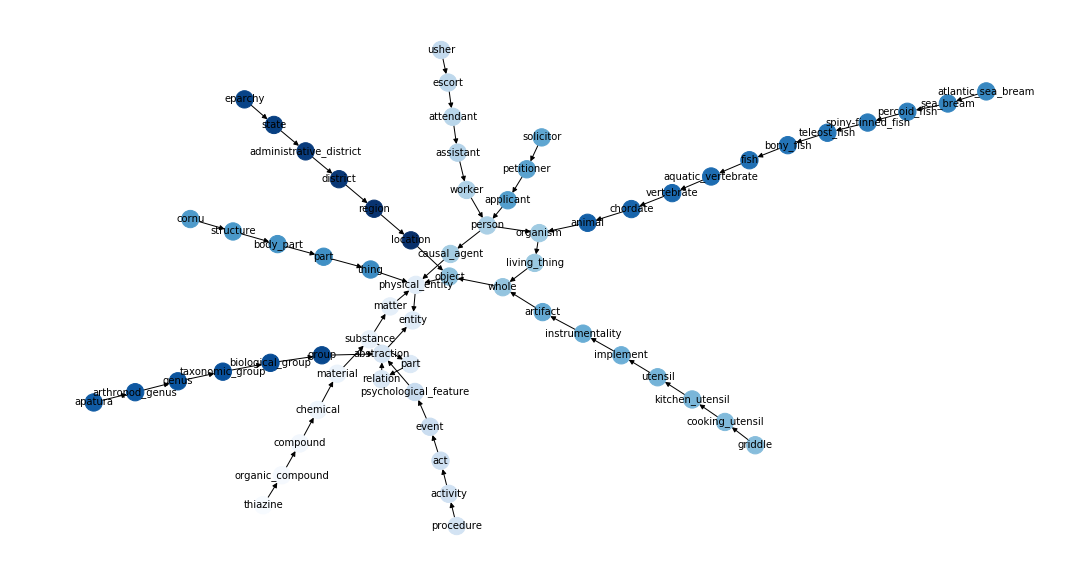
\includegraphics[width=\textwidth]{Wordnet}
\end{figure}

\begin{figure}[H]
  	\caption{Freebase Entity and Relations Graphplot}
   	\centering
    	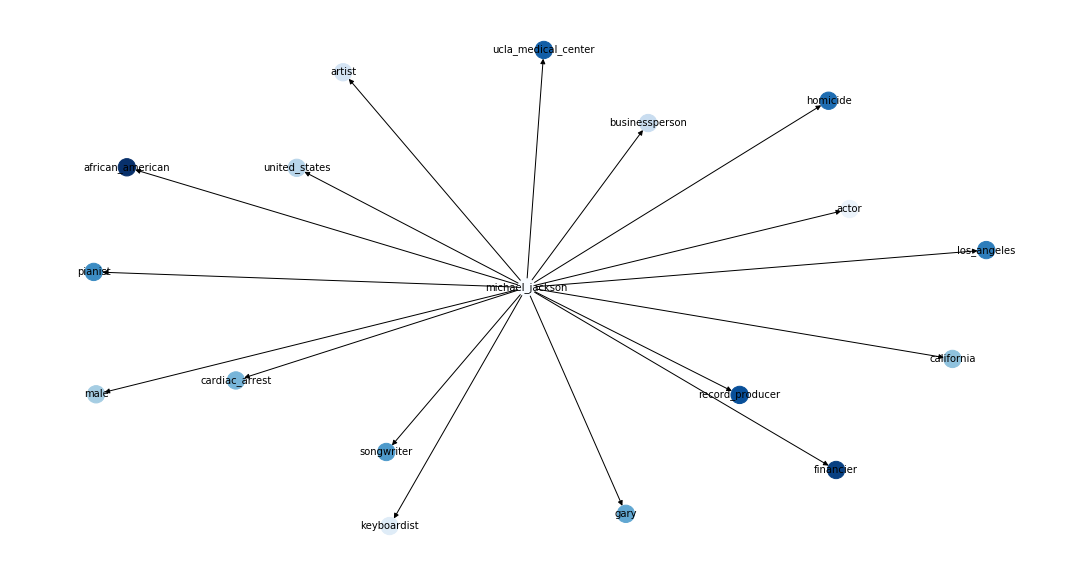
\includegraphics[width=\textwidth]{Freebase}
\end{figure}


We used the Tensorflow framework to develop our model.  This model is built on top of the Neural Tensor model introduced by (Socher, Chen, Manning and Ng 2013) ~\citep{NIPS2013_5028} and implemented in Tensorflow by (Doss, LeNail and Liu 2015)  ~\citep{Doss2015}. Randomly initialised entity and relational embeddings are used to initialise model training. These embeddings are dynamically adjusted during the training process to generate latent representations specific to the knowledge domain. Property counts for the respective knowledge graphs are presented below:

\begin{figure}[H]
	\parbox{.5\linewidth}{
   		\caption{Wordnet Property Barplot}
   		\centering
    		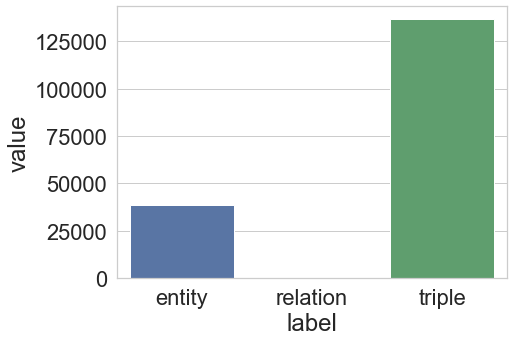
\includegraphics[width=0.45\textwidth]{Wordnet_Counts}
		}
	\hfill
	\parbox{.5\linewidth}{
		\caption{Freebase Property Barplot}
   		\centering
    		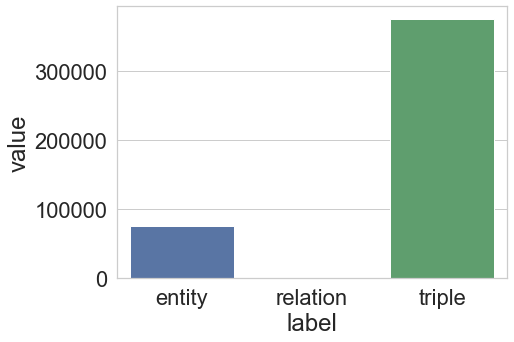
\includegraphics[width=0.45\textwidth]{Freebase_Counts}
		}
\end{figure}


\begin{table}[H]
	\parbox{.5\linewidth}{
		\caption{Wordnet Property Counts}
		\centering
		\begin{tabular}{lllllllllll}
  			\textbf{Property} & \textbf{Count}  \\
  			\hline
  			Entities & 38,696  \\
  			Relations & 11  \\
  			Triples & 136,611  \\
		\end{tabular}
		}
	\hfill
	\parbox{.5\linewidth}{
		\caption{Freebase Property Counts}
		\centering
		\begin{tabular}{lllllllllll}
  			\textbf{Property} & \textbf{Count}  \\
  			\hline
  			Entities & 75,043   \\
  			Relations & 13  \\
  			Triples & 375,499  \\
		\end{tabular}
		}
\end{table}


Summary statistics of the respective knowledge graphs Resource Description Framework (RDF) decomposition - subject, predicate, object - are presented below:

% Predicate

\begin{figure}[H]
	\parbox{.5\linewidth}{
   		\caption{Wordnet Predicate Barplot}
   		\centering
    		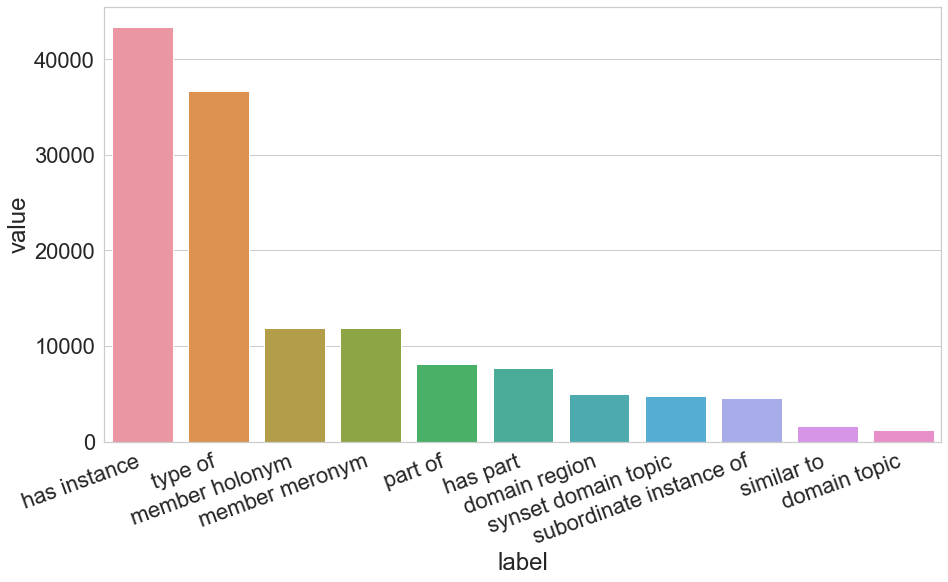
\includegraphics[width=0.45\textwidth, height=0.2\textheight]{Wordnet_Predicate_Counts}
		}
	\hfill
	\parbox{.5\linewidth}{
		\caption{Freebase Predicate Barplot}
   		\centering
		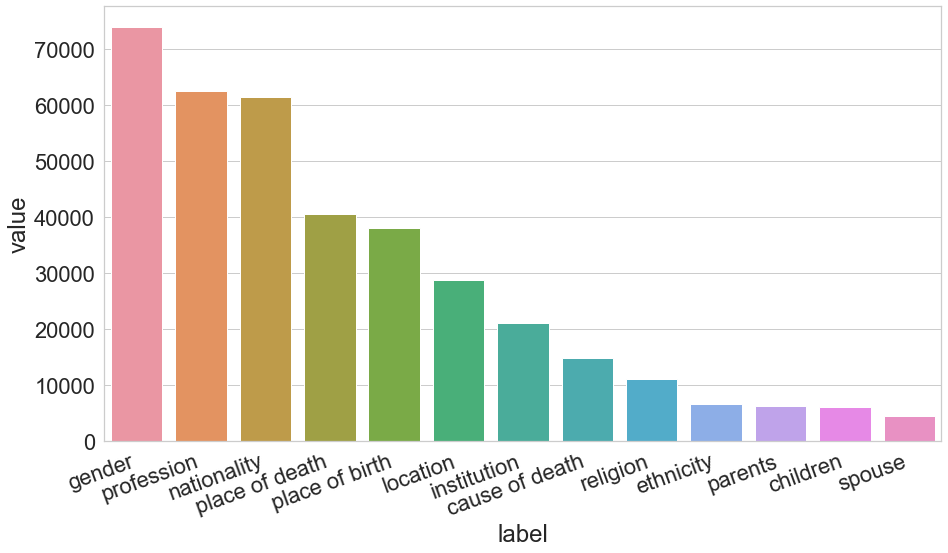
\includegraphics[width=0.45\textwidth, height=0.2\textheight]{Freebase_Predicate_Counts}
		}
\end{figure}

\begin{table}[H]
	\parbox{.5\linewidth}{
		\caption{Wordnet Predicate Statistics}
		\centering
		\begin{tabular}{lllllllllll}
  			\textbf{Statistic} & \textbf{Value}  \\
  			\hline
			Count & 11 \\
			Max & 43,312  \\
			Min & 1,229  \\
  			Median & 7,705  \\
  			IQR & 7,257.5  \\
		\end{tabular}
		}
	\hfill
	\parbox{.5\linewidth}{
		\caption{Freebase Predicate Statistics}
		\centering
		\begin{tabular}{lllllllllll}
  			\textbf{Statistic} & \textbf{Value}  \\
  			\hline
			Count & 13 \\
			Max & 73,897  \\
			Min & 4, 464  \\
  			Median & 21,149  \\
  			IQR & 34,033  \\
		\end{tabular}
		}
\end{table}

% Subject

\begin{figure}[H]
	\parbox{.5\linewidth}{
   		\caption{Wordnet Subject Barplot}
   		\centering
    		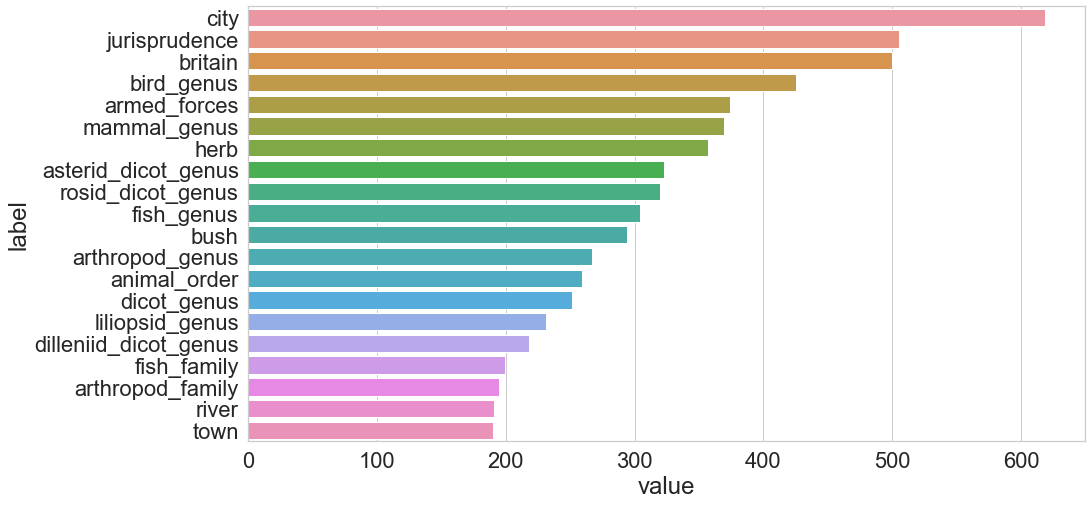
\includegraphics[width=0.45\textwidth, height=0.2\textheight]{Wordnet_Subject_Counts}
		}
	\hfill
	\parbox{.5\linewidth}{
		\caption{Freebase Subject Barplot}
   		\centering
		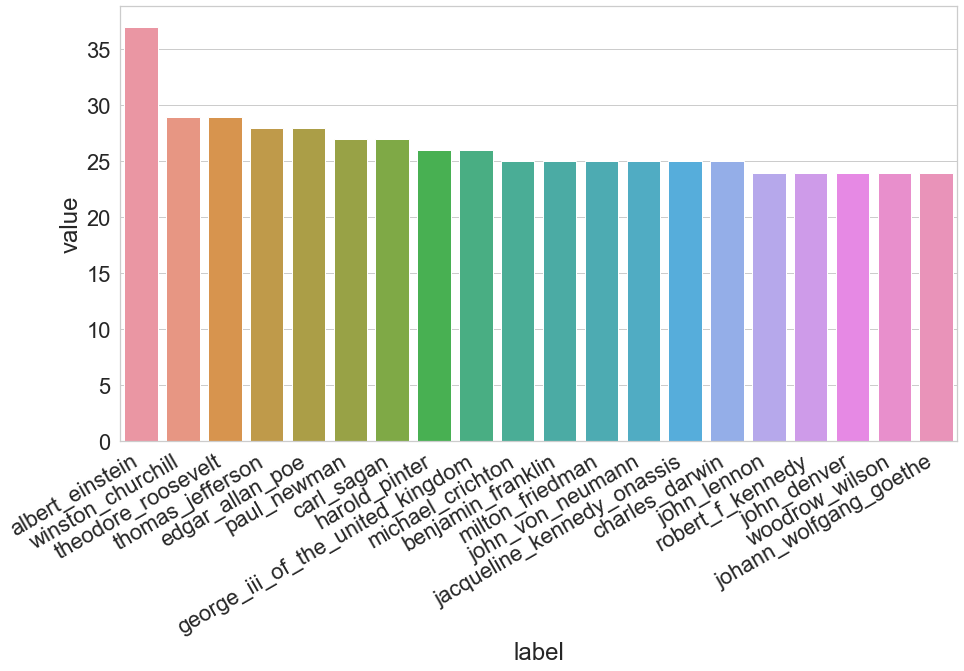
\includegraphics[width=0.45\textwidth, height=0.2\textheight]{Freebase_Subject_Counts}
		}
\end{figure}


\begin{table}[H]
	\parbox{.5\linewidth}{
		\caption{Wordnet Subject Statistics}
		\centering
		\begin{tabular}{lllllllllll}
  			\textbf{Statistic} & \textbf{Value}  \\
  			\hline
			Count & 32,720 \\
			Max & 619 \\
			Min & 1 \\
  			Median & 2 \\
  			IQR & 2 \\
		\end{tabular}
		}
	\hfill
	\parbox{.5\linewidth}{
		\caption{Freebase Subject Statistics}
		\centering
		\begin{tabular}{lllllllllll}
  			\textbf{Statistic} & \textbf{Value}  \\
  			\hline
			Count & 67,393 \\
			Max & 37 \\
			Min & 1 \\
  			Median & 5 \\
  			IQR & 4 \\
		\end{tabular}
		}
\end{table}

% Object

\begin{figure}[H]
	\parbox{.5\linewidth}{
   		\caption{Wordnet Object Barplot}
   		\centering
    		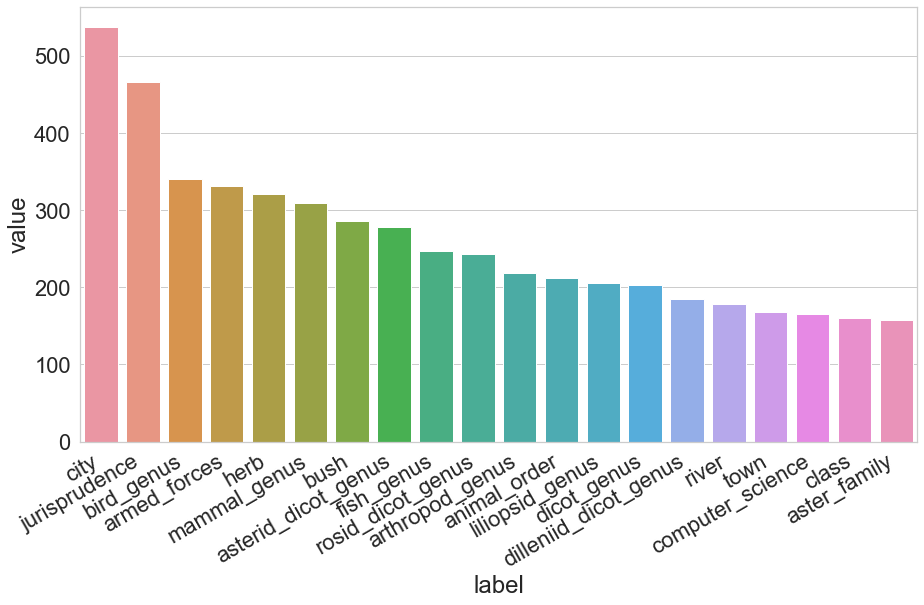
\includegraphics[width=0.45\textwidth, height=0.2\textheight]{Wordnet_Object_Counts}
		}
	\hfill
	\parbox{.5\linewidth}{
		\caption{Freebase Object Barplot}
   		\centering
		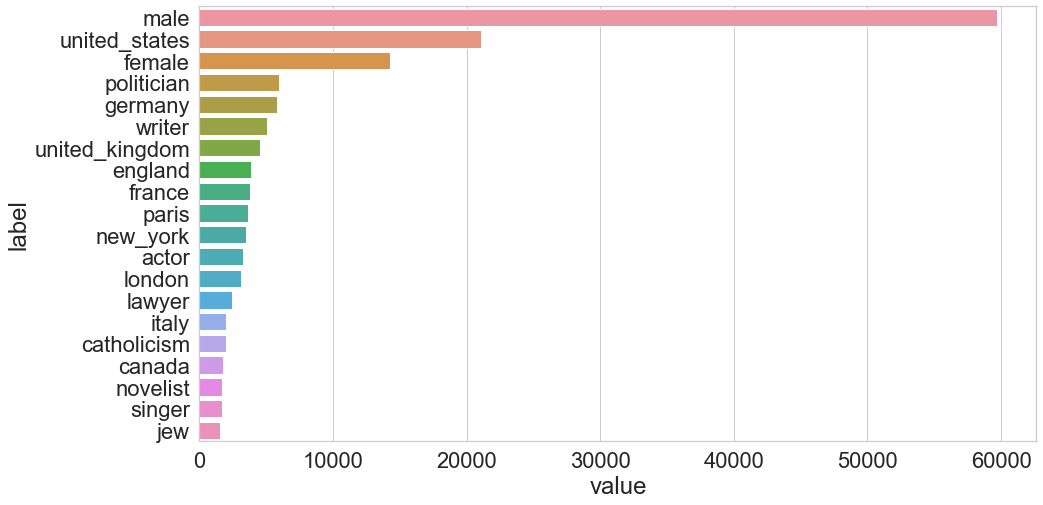
\includegraphics[width=0.45\textwidth, height=0.2\textheight]{Freebase_Object_Counts}
		}
\end{figure}


\begin{table}[H]
	\parbox{.5\linewidth}{
		\caption{Wordnet Object Statistics}
		\centering
		\begin{tabular}{lllllllllll}
  			\textbf{Statistic} & \textbf{Value}  \\
  			\hline
			Count & 33,011 \\
			Max & 537 \\
			Min & 1 \\
  			Median & 3 \\
  			IQR & 2 \\
		\end{tabular}
		}
	\hfill
	\parbox{.5\linewidth}{
		\caption{Freebase Object Statistics}
		\centering
		\begin{tabular}{lllllllllll}
  			\textbf{Statistic} & \textbf{Value}  \\
  			\hline
			Count & 15,342 \\
			Max & 59,663 \\
			Min & 1 \\
  			Median & 3 \\
  			IQR & 6 \\
		\end{tabular}
		}
\end{table}

For Wordnet, it can be seen that relations are skewed toward "has instance" 43,312 occurrences, and "type of" 36,659 occurrences. We would expect poor performance from the model for out-of-sample data containing
containing relations that are not "has instance" or "type of". Freebase relations are somewhat more uniform, however four relations have occurrences under 10,000. We would expect reasonable performance across all relations for this knowledge graph. \newline
Wordnet and Freebae subjects are somewhat uniform, although the median number of occurrences is 2 and 5 respectively, with an IQR of 2 and 4 respectively. This are thus sparse distributions of data points, and the model will need to rely on 
similarity of subject features in order to produce sensible inference. \newline
Wordnet object occurrences are somewhat uniform. Freebase object occurrences are skewed, with a single object, "male" occurring 59,663 times, representing 15,88\% of facts. This is in comparison to a median object occurrence of 3 and an interquartile range of 6.
We would expect poor performance from a Freebase link prediction model given this distribution of objects. \newline

% Best Practise Deep Learning Techniques

\subsubsection{Hypothesis 1: \newline 
Recursive Neural Tensor Networks with Best Practise Deep Learning Techniques}
Model hyperparameter optimisation is implemented using random grid search. The the model was trained on a MacBook Pro 2015 with 8 cores, 16GB RAM, and 512GB SSD. \newline
We evaluate the model by ranking the accuracy scores of the predicted triples for the respective datasets. Code to reproduce: https://github.com/xhosaBoy/deep-knowledge-modelling

\subsubsection{Batching, Logits and Early Stopping}
Machine learning models can suffer from overfitting \cite{reference} - when training has progressed too long, and the model parameters have been optimised for prediction on the training set. This leads to poor generalisation  and reveals itself in the form of increasing training accuracy, and decreasing validation accuracy. In order to overcome this problem, early stopping is often used during training. This is when triaining is terminated should decreasing validation accuracy be detected.\newline

\subsubsection{Link Prediction Results}
The link prediction accuracy results of the RNTN model, a nonlinear factorisation model compared against linear factorisation models, are presented in table 5.1:

\begin{figure}[H]
	\parbox{.5\linewidth}{
   		\caption{Wordnet Cost}
   		\centering
    		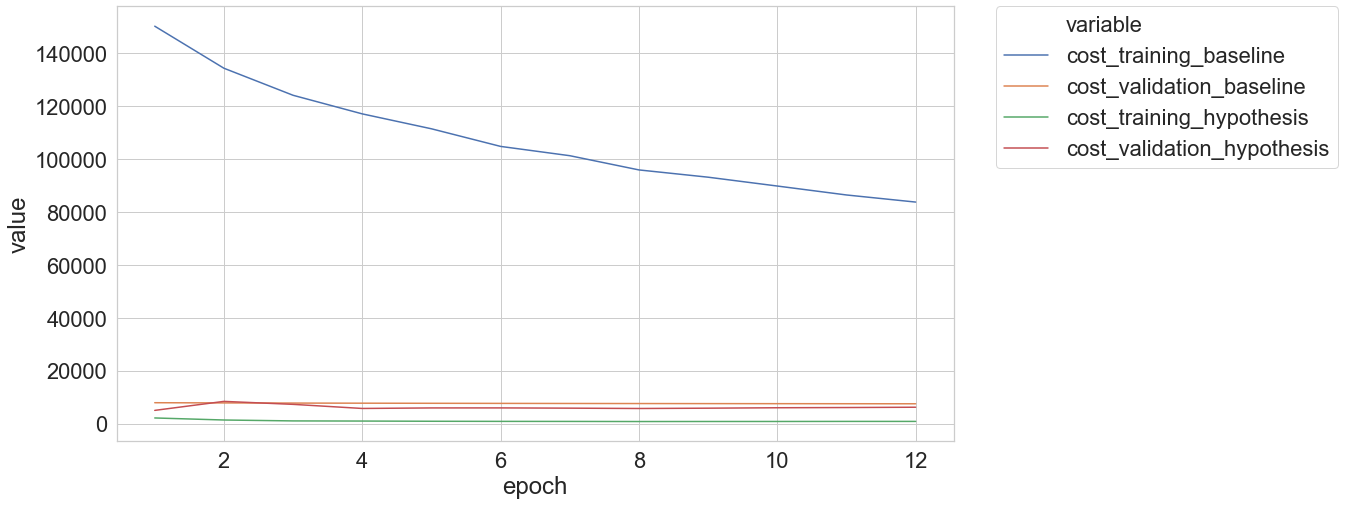
\includegraphics[width=0.45\textwidth, height=0.2\textheight]{Wordnet_Cost_Results_Early_Stopping}
		}
	\hfill
	\parbox{.5\linewidth}{
		\caption{Freebase Cost}
   		\centering
		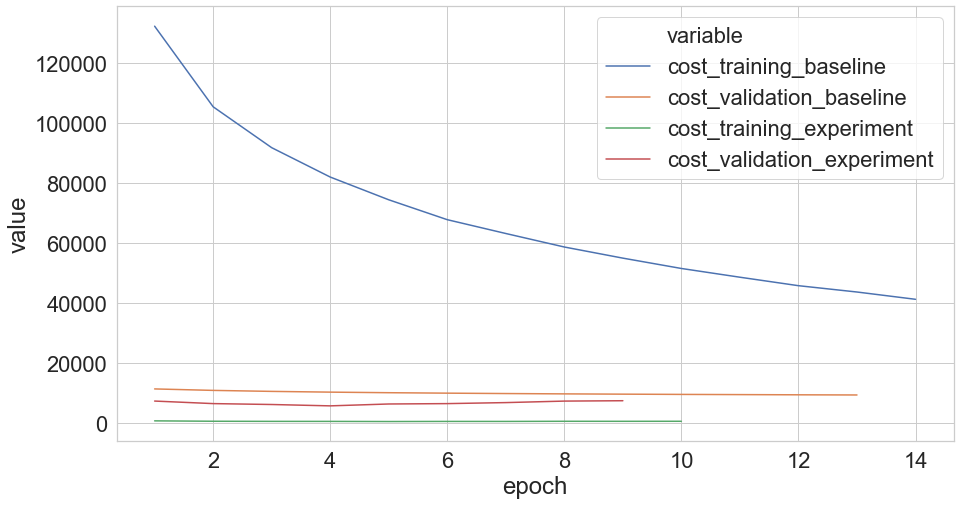
\includegraphics[width=0.45\textwidth, height=0.2\textheight]{Freebase_Cost_Results}
		}
\end{figure}


\begin{figure}[H]
	\parbox{.5\linewidth}{
   		\caption{Wordnet Accuracy}
   		\centering
    		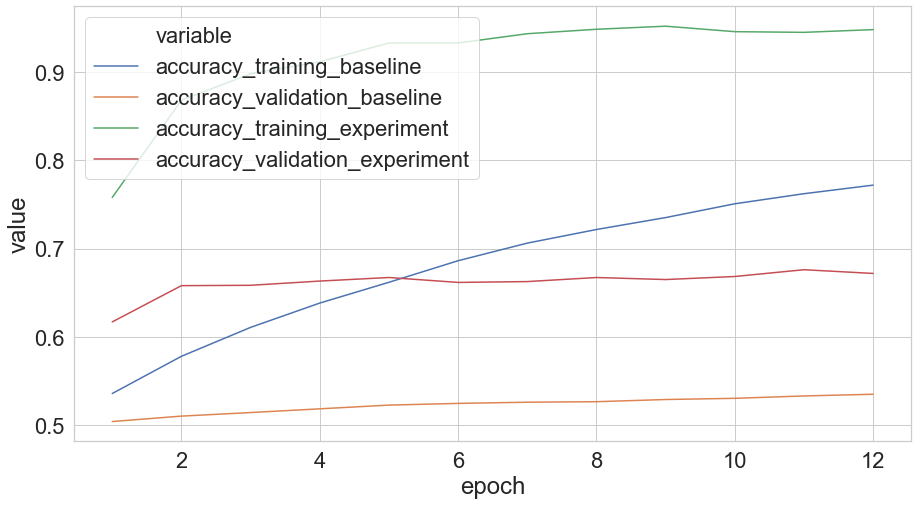
\includegraphics[width=0.45\textwidth, height=0.2\textheight]{Wordnet_Accuracy_Results_Early_Stopping}
		}
	\hfill
	\parbox{.5\linewidth}{
		\caption{Freebase Accuracy}
   		\centering
		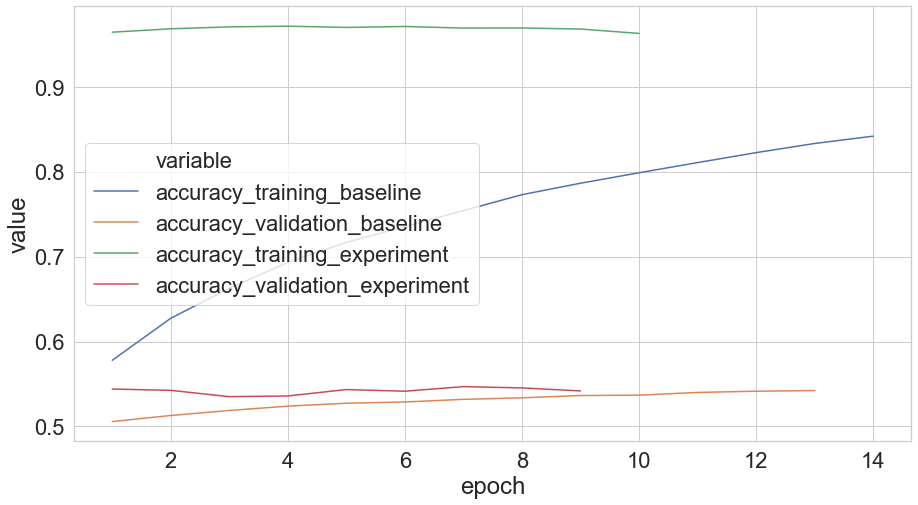
\includegraphics[width=0.45\textwidth, height=0.2\textheight]{Freebase_Accuracy_Results}
		}
\end{figure}



\begin{table}[H]
	\caption{Link prediction accuracy on Wordnet and Freebase}
	\centering
	\begin{tabular}{lllllllllll}
  		\textbf{Model} & \textbf{Wordnet} & \textbf{Freebbase} & \textbf{Avg} \\
  		\hline
  		Distance Model & .683 & .610 & .647 \\
  		Hadamard Model & .800 & .688 & .744 \\
  		Single Layer Model & .760 & .853 & .807 \\
  		Bilinear Model & \textbf{.841} & \textbf{.877} & \textbf{.859} \\
  		Recursive Neural Tensor Network & .562 & .535 & .549 \\
  		\hline
  		Recursive Neural Tensor Network+ & .674 & .548 & .611 \\
	\end{tabular}
\end{table}

\section{HypER Convolutional Neural Networks}

\subsubsection{Model Summary} 
In order to overcome the expressiveness problems evident in the Freebase test dataset, more nonlinear relational factorisation approaches have been proposed \cite{ComplEx, Neural LP, TorusE}. \newline
HypER is a model that uses convolutional relational filters r that are convolved with the subject entity e1, producing an intermediate relational representation. The dot product of the relational representation is then taken with the object entity e2 to produce relation-specific score between the two entities. The HypER model only produces a latent relational representation for the subject entity e1, we extend this model to also produce a relational representation for the object entity e2, and call this model HpyER+. HypER+ thus produces entity-relational representations that approximate KG spacial locality. \newline
\subsubsection{Binary Cross Entropy Loss}
The binary cross entropy loss \cite{reference} is used to train the HypER Convolutional model. Like the RNTN model, the input consists of an entity-relational pair, where the entity is a subject entity and an object entity is presented as a target to complete the triple. A logit is generated for each sample and passed through through a logarithmic sigmoid or softmax function. Loss is generated by comparing the produced likelihood with the expected likelihood, 0 or 1. The sum of all losses is aggregated and back propagated through the network for parameter update. \newline

\subsubsection{Experimental Setup} 

We use the following benchmark knowledge graphs: WN18 (Bordes et al. 2013) is a subset of Wordnet, a database containing lexical relations between words. The knowledge graph contains 40,943 entities and 18 relations. \newline 
FB15k - (Bordes et al. 2013) is a subset of Freebase, a large database of facts about the real world. FB15k contains 14,951 entities and 1,345 relations. \newline \newline
Visualisations of the respective knowledge graphs are presented below:

\begin{figure}[H]
  	\caption{WN18 Entities and Relations Graphplot}
   	\centering
    	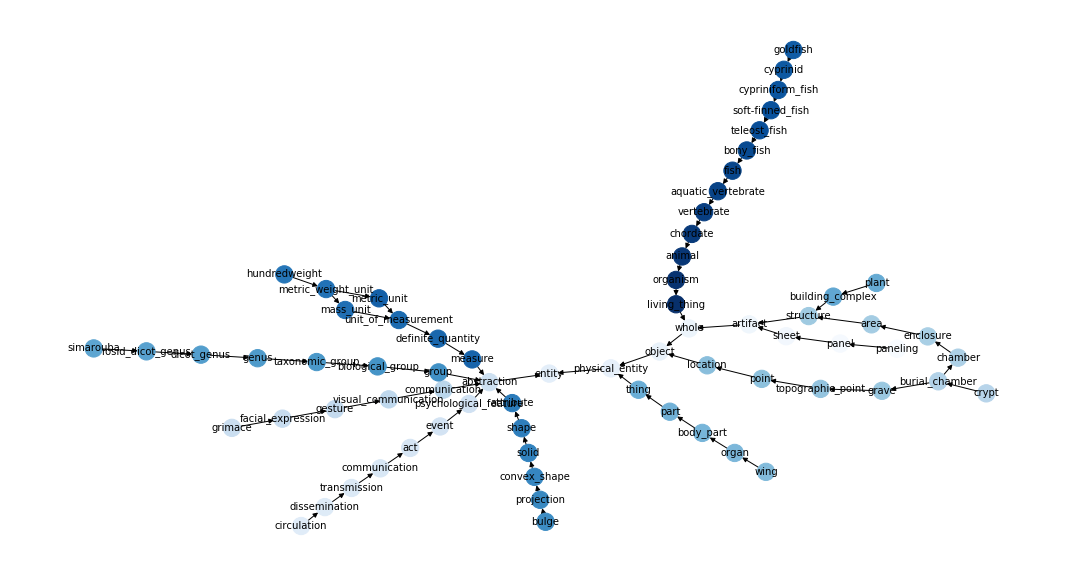
\includegraphics[width=\textwidth]{WN18_Graph}
\end{figure}

\begin{figure}[H]
  	\caption{FB15k Entity and Relations Graphplot}
   	\centering
    	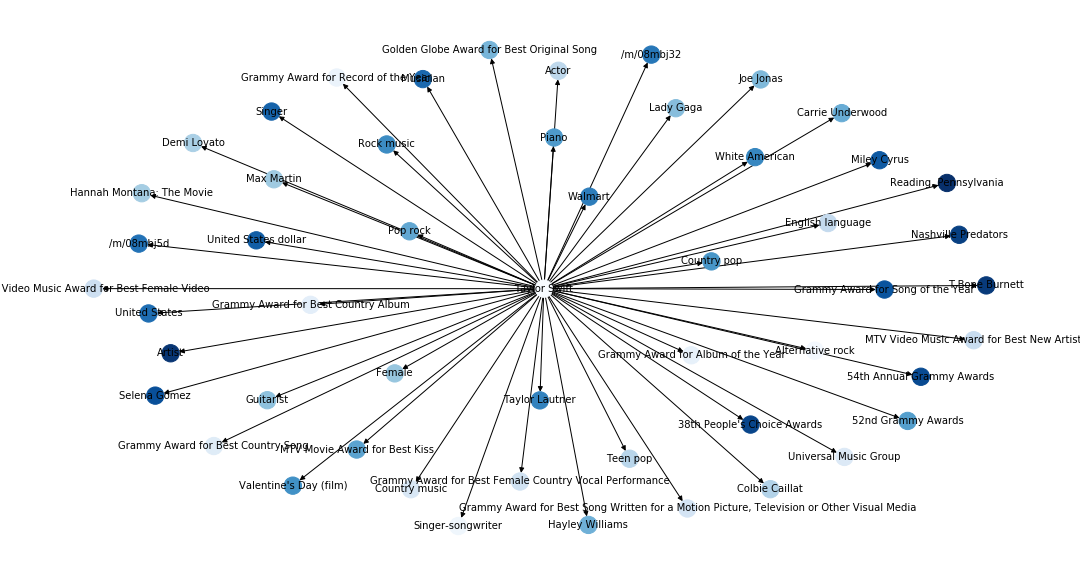
\includegraphics[width=\textwidth]{FB15k_Graph}
\end{figure}


We used the Pytorch framework to develop our model. This model is built on top of the HypER model introduced by (Balaˇzevi´c, Allen, and Hospedales 2018) ~\citep{balazevic2019hypernetwork}.  Randomly initialised entity and relational embeddings are used to initialise model training. These embeddings are dynamically adjusted during the training process to generate latent representations specific to the knowledge domain. Property counts for the respective knowledge graphs are presented below:

\begin{figure}[H]
	\parbox{.5\linewidth}{
   		\caption{WN18 Property Barplot}
   		\centering
    		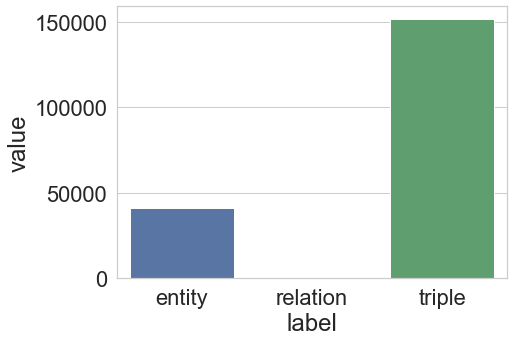
\includegraphics[width=0.45\textwidth]{WN18_Counts}
		}
	\hfill
	\parbox{.5\linewidth}{
		\caption{FB15k Property Barplot}
   		\centering
    		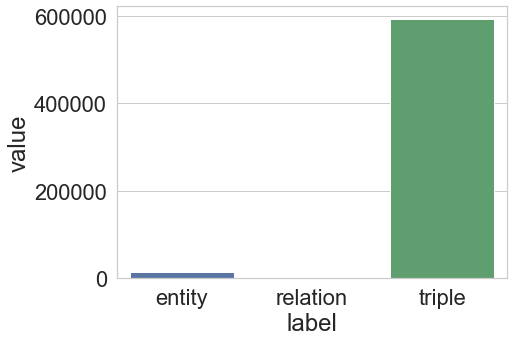
\includegraphics[width=0.45\textwidth]{FB15k_Counts}
		}
\end{figure}


\begin{table}[H]
	\parbox{.5\linewidth}{
		\caption{WN18 Property Counts}
		\centering
		\begin{tabular}{lllllllllll}
  			\textbf{Property} & \textbf{Count}  \\
  			\hline
  			Entities & 40,943  \\
  			Relations & 18  \\
  			Triples & 151,442 \\
		\end{tabular}
		}
	\hfill
	\parbox{.5\linewidth}{
		\caption{FB15k Property Counts}
		\centering
		\begin{tabular}{lllllllllll}
  			\textbf{Property} & \textbf{Count}  \\
  			\hline
  			Entities & 14,951   \\
  			Relations & 1,345  \\
  			Triples & 592,213  \\
		\end{tabular}
		}
\end{table}


Summary statistics of the respective knowledge graphs Resource Description Framework (RDF) decomposition - subject, predicate, object - are presented below:

% Predicate

\begin{figure}[H]
	\parbox{.5\linewidth}{
   		\caption{WN18 Predicate Barplot}
   		\centering
    		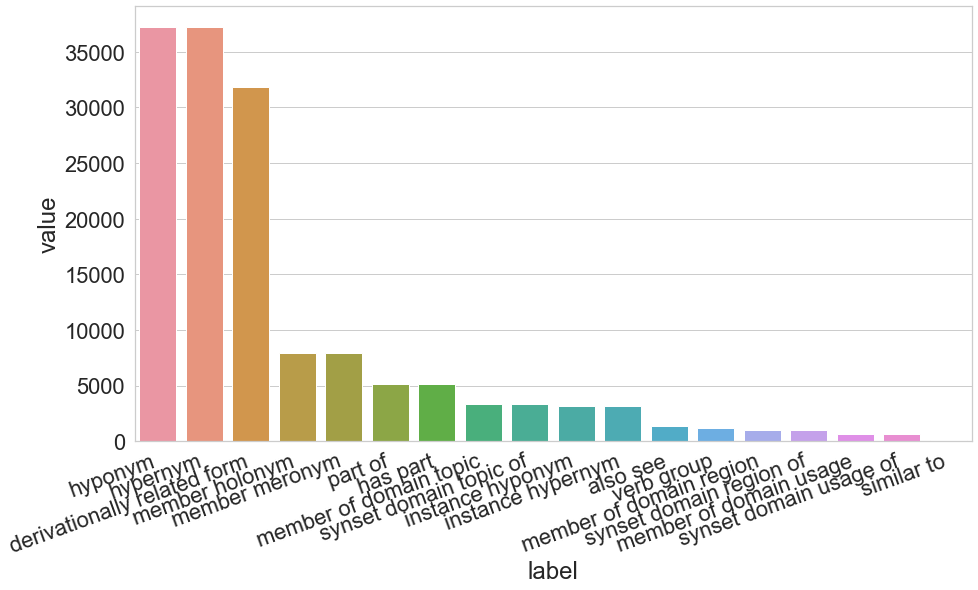
\includegraphics[width=0.45\textwidth, height=0.2\textheight]{WN18_Predicate_Counts}
		}
	\hfill
	\parbox{.5\linewidth}{
		\caption{FB15k Predicate Barplot}
   		\centering
		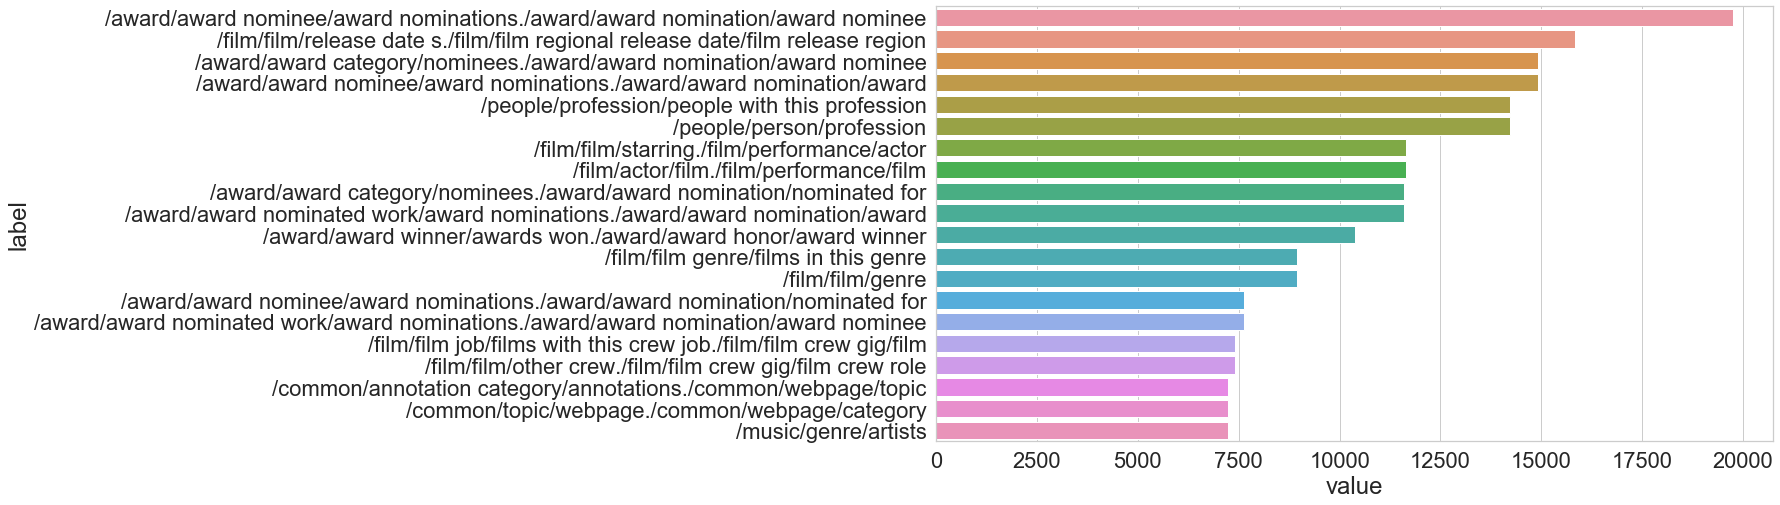
\includegraphics[width=0.45\textwidth, height=0.2\textheight]{FB15k_Predicate_Counts}
		}
\end{figure}

\begin{table}[H]
	\parbox{.5\linewidth}{
		\caption{WN18 Predicate Statistics}
		\centering
		\begin{tabular}{lllllllllll}
  			\textbf{Statistic} & \textbf{Value}  \\
  			\hline
			Count & 18 \\
			Max & 37,221  \\
			Min & 86 \\
  			Median & 3,242.5  \\
  			IQR & 6,190.75  \\
		\end{tabular}
		}
	\hfill
	\parbox{.5\linewidth}{
		\caption{FB15k Predicate Statistics}
		\centering
		\begin{tabular}{lllllllllll}
  			\textbf{Statistic} & \textbf{Value}  \\
  			\hline
			Count & 1,345 \\
			Max & 19,764  \\
			Min & 1  \\
  			Median & 26  \\
  			IQR & 166  \\
		\end{tabular}
		}
\end{table}

% Subject

\begin{figure}[H]
	\parbox{.5\linewidth}{
   		\caption{WN18 Subject Barplot}
   		\centering
    		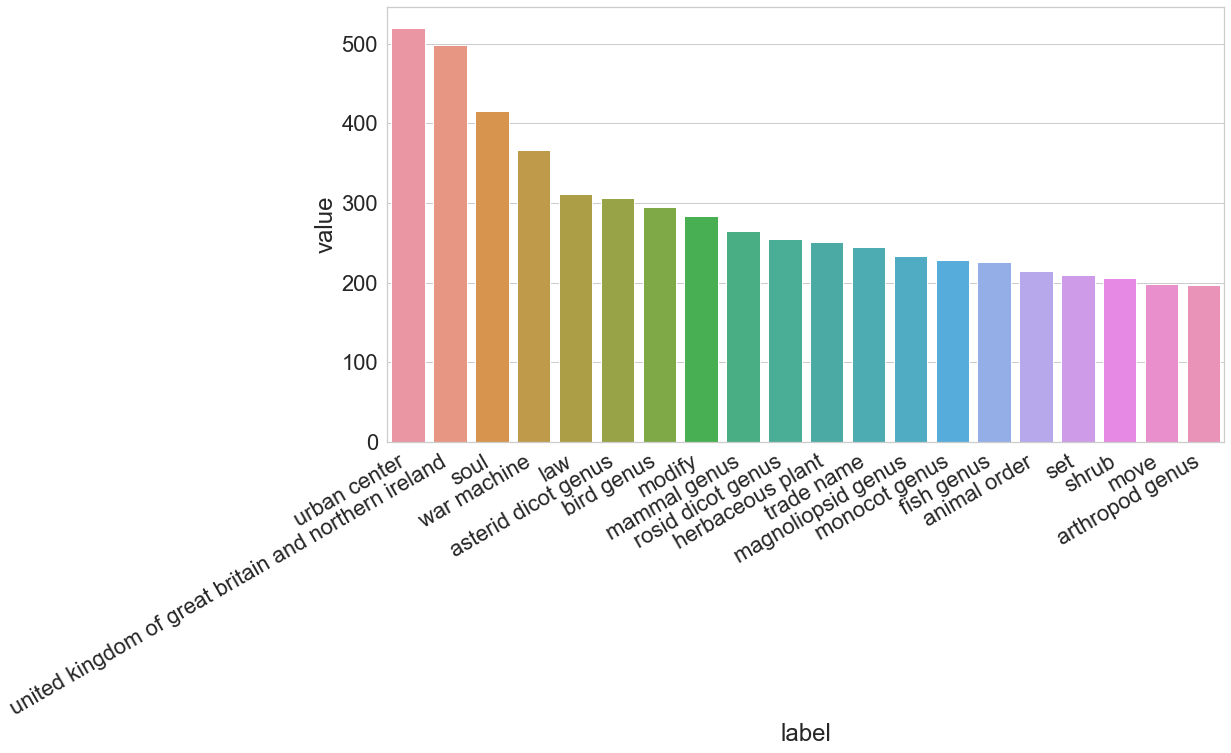
\includegraphics[width=0.45\textwidth, height=0.2\textheight]{WN18_Subject_Counts}
		}
	\hfill
	\parbox{.5\linewidth}{
		\caption{FB15k Subject Barplot}
   		\centering
		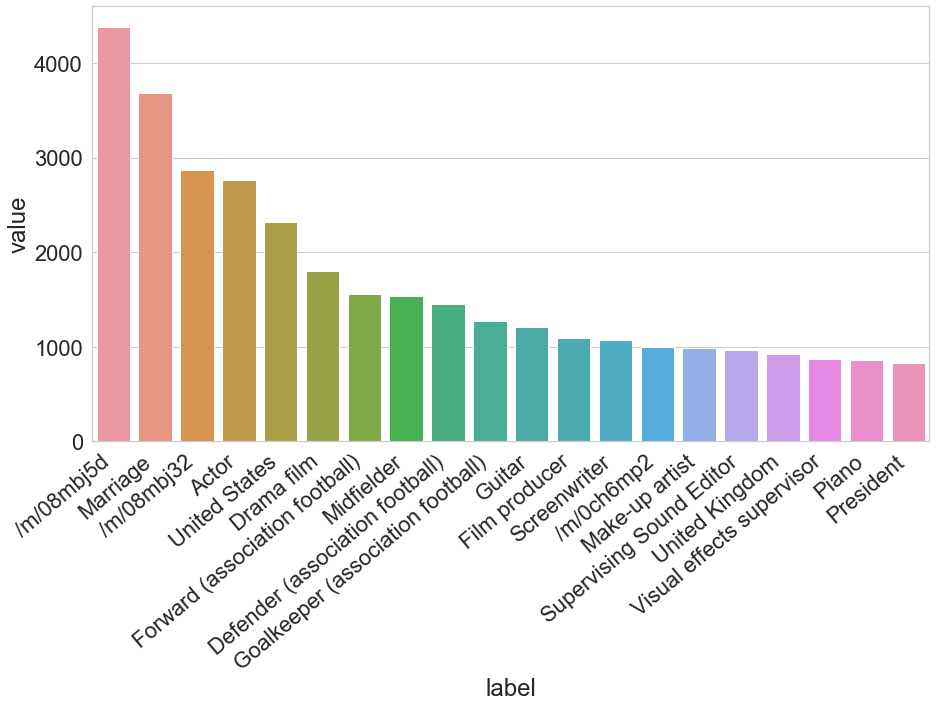
\includegraphics[width=0.45\textwidth, height=0.2\textheight]{FB15k_Subject_Counts}
		}
\end{figure}


\begin{table}[H]
	\parbox{.5\linewidth}{
		\caption{WN18 Subject Statistics}
		\centering
		\begin{tabular}{lllllllllll}
  			\textbf{Statistic} & \textbf{Value}  \\
  			\hline
			Count & 32,544 \\
			Max & 520 \\
			Min & 1 \\
  			Median & 3 \\
  			IQR & 2 \\
		\end{tabular}
		}
	\hfill
	\parbox{.5\linewidth}{
		\caption{FB15k Subject Statistics}
		\centering
		\begin{tabular}{lllllllllll}
  			\textbf{Statistic} & \textbf{Value}  \\
  			\hline
			Count &14,865 \\
			Max & 4,381 \\
			Min & 1 \\
  			Median & 27 \\
  			IQR & 32 \\
		\end{tabular}
		}
\end{table}

% Object

\begin{figure}[H]
	\parbox{.5\linewidth}{
   		\caption{WN18 Object Barplot}
   		\centering
    		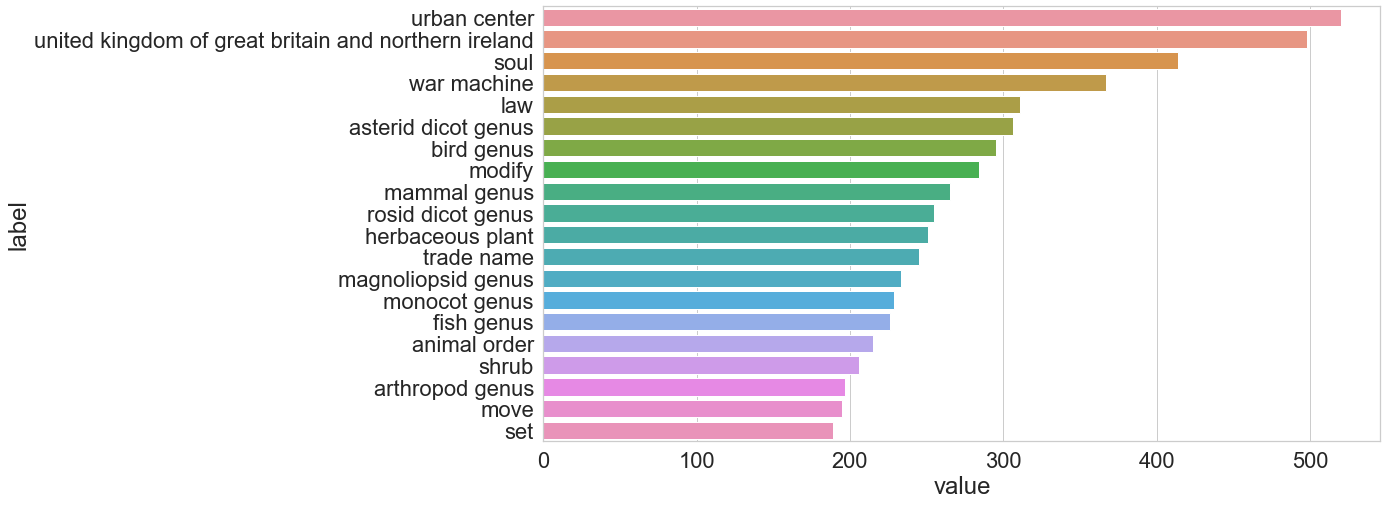
\includegraphics[width=0.45\textwidth, height=0.2\textheight]{WN18_Object_Counts}
		}
	\hfill
	\parbox{.5\linewidth}{
		\caption{FB15k Object Barplot}
   		\centering
		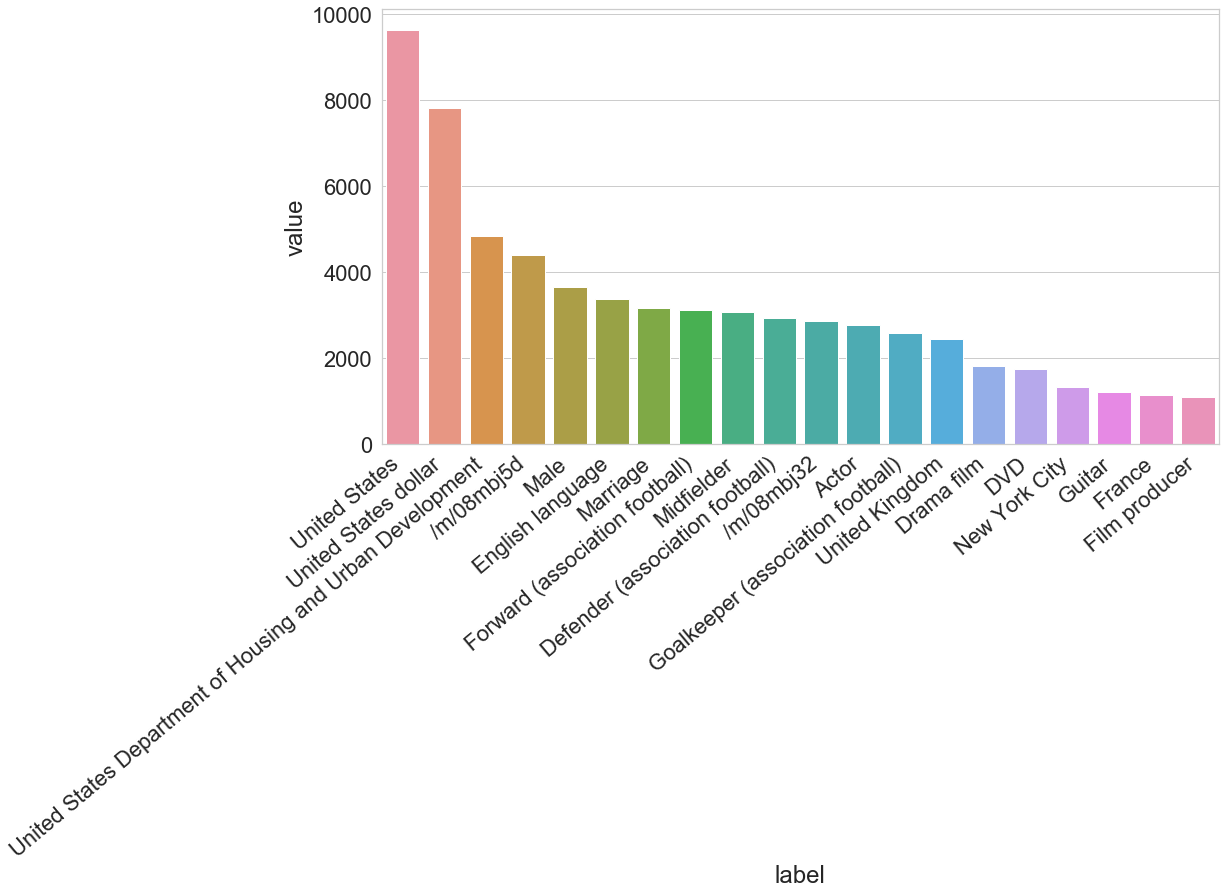
\includegraphics[width=0.45\textwidth, height=0.2\textheight]{FB15k_Object_Counts}
		}
\end{figure}


\begin{table}[H]
	\parbox{.5\linewidth}{
		\caption{WN18 Object Statistics}
		\centering
		\begin{tabular}{lllllllllll}
  			\textbf{Statistic} & \textbf{Value}  \\
  			\hline
			Count & 32,543 \\
			Max & 520 \\
			Min & 1 \\
  			Median & 3 \\
  			IQR & 2 \\
		\end{tabular}
		}
	\hfill
	\parbox{.5\linewidth}{
		\caption{FB15k Object Statistics}
		\centering
		\begin{tabular}{lllllllllll}
  			\textbf{Statistic} & \textbf{Value}  \\
  			\hline
			Count & 14,930 \\
			Max & 9,645 \\
			Min & 1 \\
  			Median & 23 \\
  			IQR & 30 \\
		\end{tabular}
		}
\end{table}

For WN18, it can be seen that relations are skewed toward the relations "hyponym",  "hypernym", and "derivationally related from", with a maximum of 37,221 occurrences. \newline
FB15k relations are somewhat more uniform. We would expect reasonable performance across all relations for this knowledge graph. \newline
WN18 and FB15k subjects are somewhat uniform aside from a small number of high occurrences entities, with the median number of occurrences is 3 and 27 respectively, and with an IQR of 2 and 32 respectively. 
WN18 object occurrences are somewhat uniform. FB15k object occurrences are skewed, with the "United States" partaking in the highest number of facts. This is in comparison to a median object occurrence of 3 and an interquartile range of 23.

%  Regularised Relational Filters

\subsubsection{Hypothesis 2: \newline 
HypER Relational Filter Regularisation: HypER+}
HypER Relational Filter Regularisation, introduced as HypER+, is implemented using regularised relational filters, as well an adjustment of hidden layer regularisation, from the original HypER model. \newline
The the model was trained on Google Cloud Platform, on a N1 series instance with  8 CPU cores, 30GB RAM, 512GB SSD and a Nvidia Tesla P100 GPU. \newline
We evaluate the model using standard link prediction benchmarks. \newline 
Code to reproduce: https://github.com/xhosaBoy/HypER-Regularised-Relations \newline
Baseline: https://github.com/xhosaBoy/HypER-baseline

\subsubsection{Dropout and Batch Normalisation}
Deep learning models are prone to overfitting training data due to over parameterisation ~\citep{dropout paper}. A technique called dropout is used to overcome this problem. 
Dropout involves removing nodes within a layer, to remove excessive dependency on that node by the model. This encourages generalisation by the model, to the underlying distribution of the data. \newline  
Datasets often suffer from noise. This noise masks the true underlying distribution of the data, and can make it challenging for a model to estimate the likely distribution.
An aggregation of data samples help reveal the true distribution ~\citep{Book about statistical machine learning}. Batch nomralisation is the application of statistical properties of such a data aggregation
to individual data points within a dataset. Typically the mean and standard deviation of the bath is applied to a batch that will be used to compute forward and back propagation through the network. \newline
This technique is applied to relational filters in the HypER model. Batch normalisaiton is already applied to entity data points in the model. 

\subsubsection{Link Prediction Results}
The link prediction benchmark results of the HypER+ model, compared against other link prediction models, are presented below:

% Cost

\begin{figure}[H]
	\parbox{.5\linewidth}{
   		\caption{WN18 Cost}
   		\centering
    		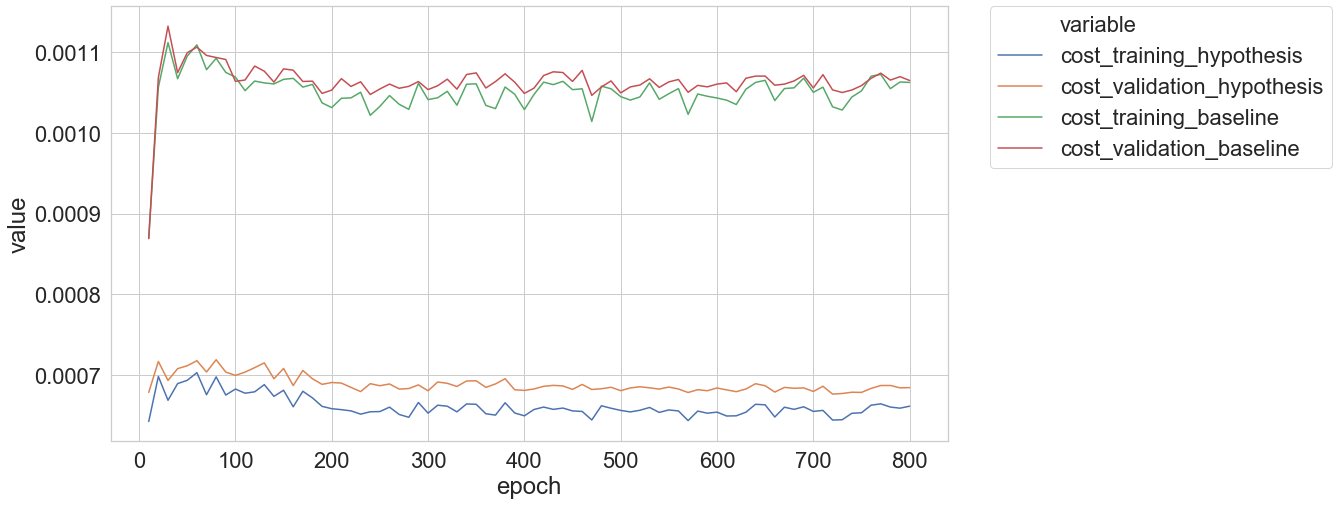
\includegraphics[width=0.45\textwidth, height=0.2\textheight]{WN18_Cost_Results}
		}
	\hfill
	\parbox{.5\linewidth}{
		\caption{FB15k Cost}
   		\centering
		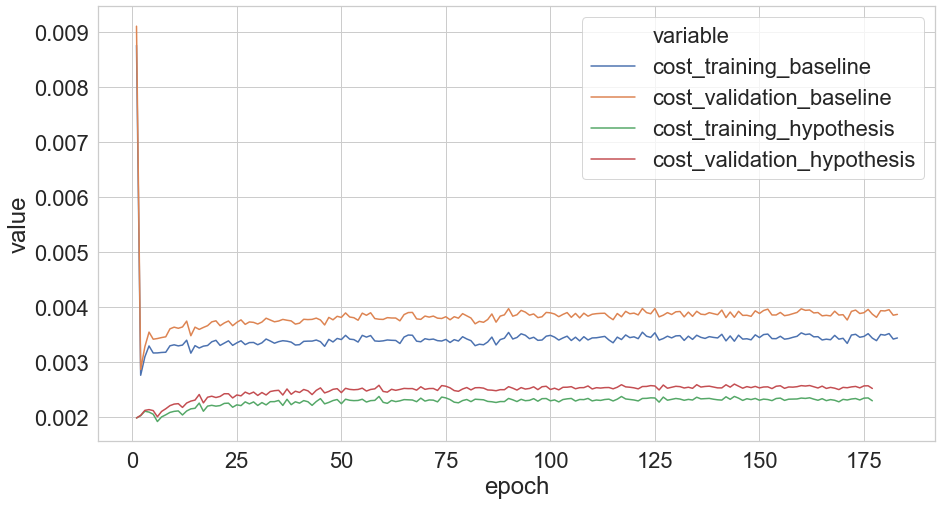
\includegraphics[width=0.45\textwidth, height=0.2\textheight]{FB15k_Cost_Results}
		}
\end{figure}

\begin{figure}[H]
	\parbox{.5\linewidth}{
   		\caption{WN18 Cost Clipped View}
   		\centering
    		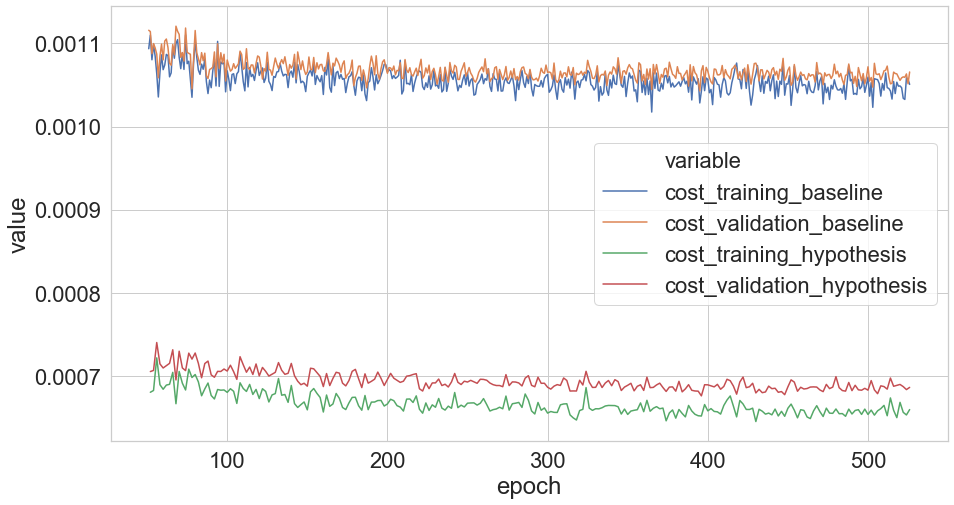
\includegraphics[width=0.45\textwidth, height=0.2\textheight]{WN18_Cost_Results_Clipped}
		}
	\hfill
	\parbox{.5\linewidth}{
		\caption{FB15k Cost Clipped View}
   		\centering
		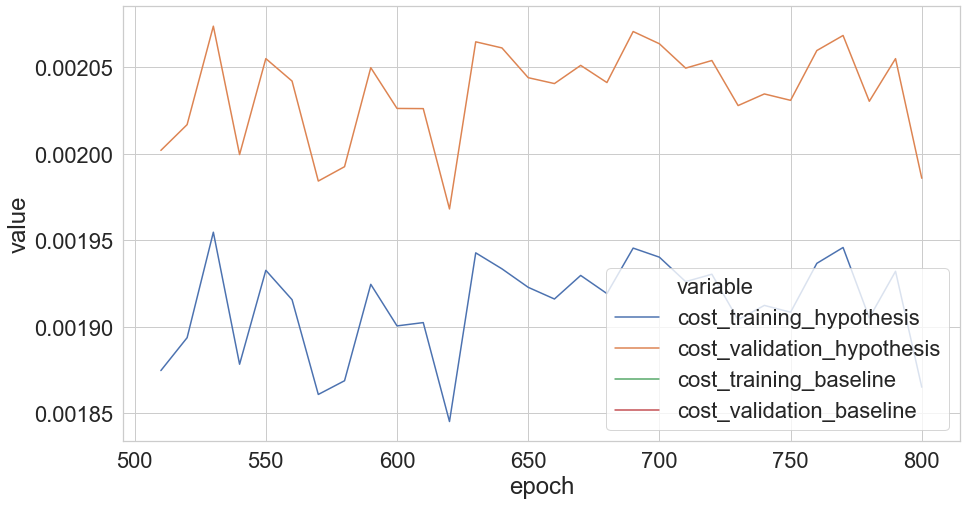
\includegraphics[width=0.45\textwidth, height=0.2\textheight]{FB15k_Cost_Results_Clipped}
		}
\end{figure}

% Hits@10

\begin{figure}[H]
	\parbox{.5\linewidth}{
   		\caption{WN18 Hits@10}
   		\centering
    		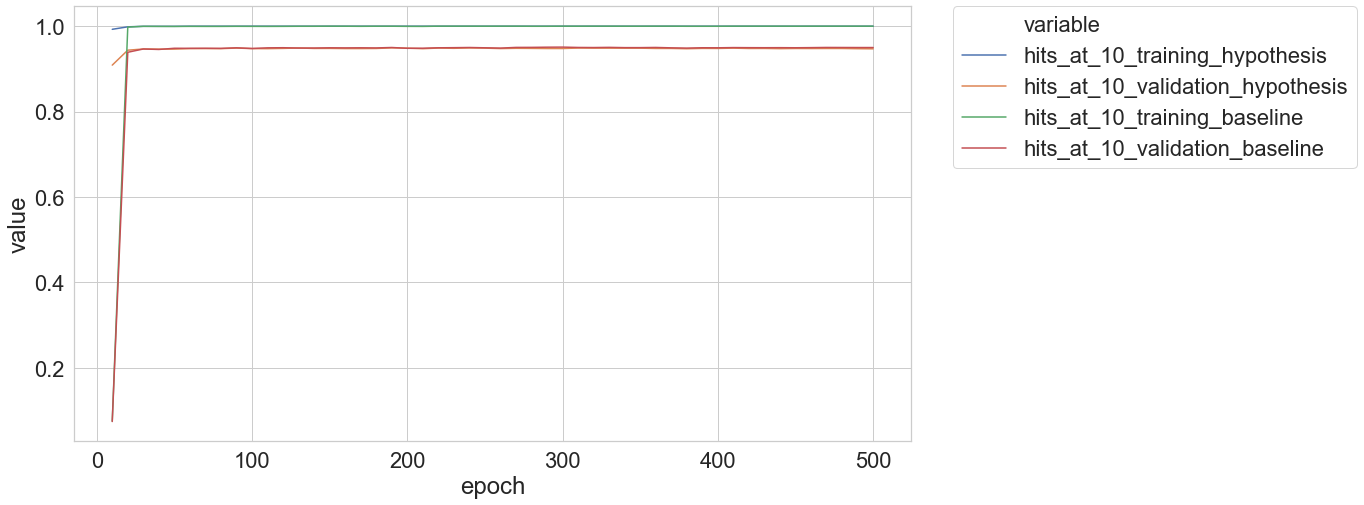
\includegraphics[width=0.45\textwidth, height=0.2\textheight]{WN18_hits_at_10_Results}
		}
	\hfill
	\parbox{.5\linewidth}{
		\caption{FB15k Hits@10}
   		\centering
		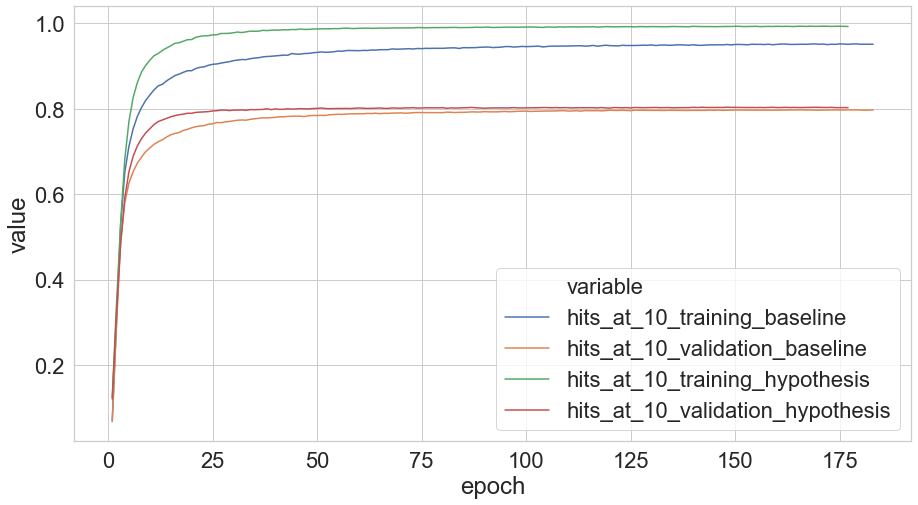
\includegraphics[width=0.45\textwidth, height=0.2\textheight]{FB15k_hits_at_10_Results}
		}
\end{figure}

\begin{figure}[H]
	\parbox{.5\linewidth}{
   		\caption{WN18 Hits@10 Clipped View}
   		\centering
    		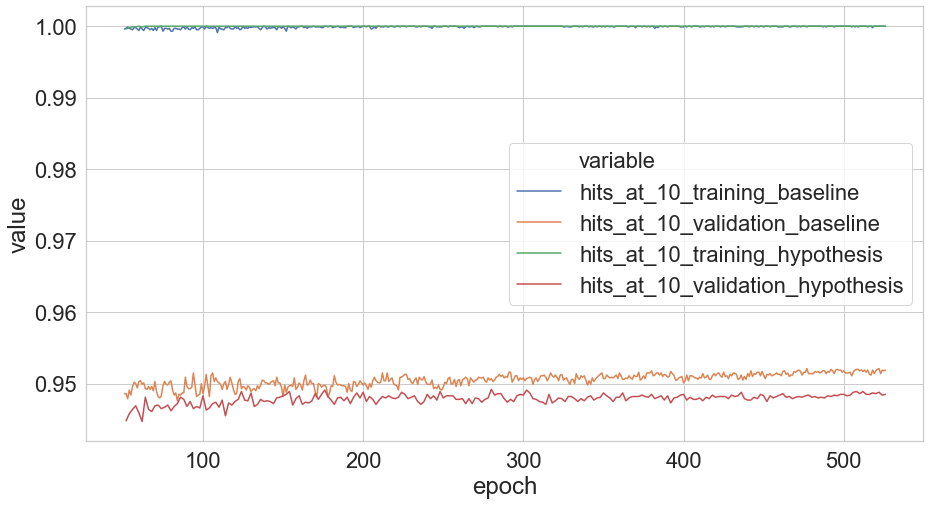
\includegraphics[width=0.45\textwidth, height=0.2\textheight]{WN18_hits_at_10_Results_Clipped}
		}
	\hfill
	\parbox{.5\linewidth}{
		\caption{FB15k Hits@10  Clipped View}
   		\centering
		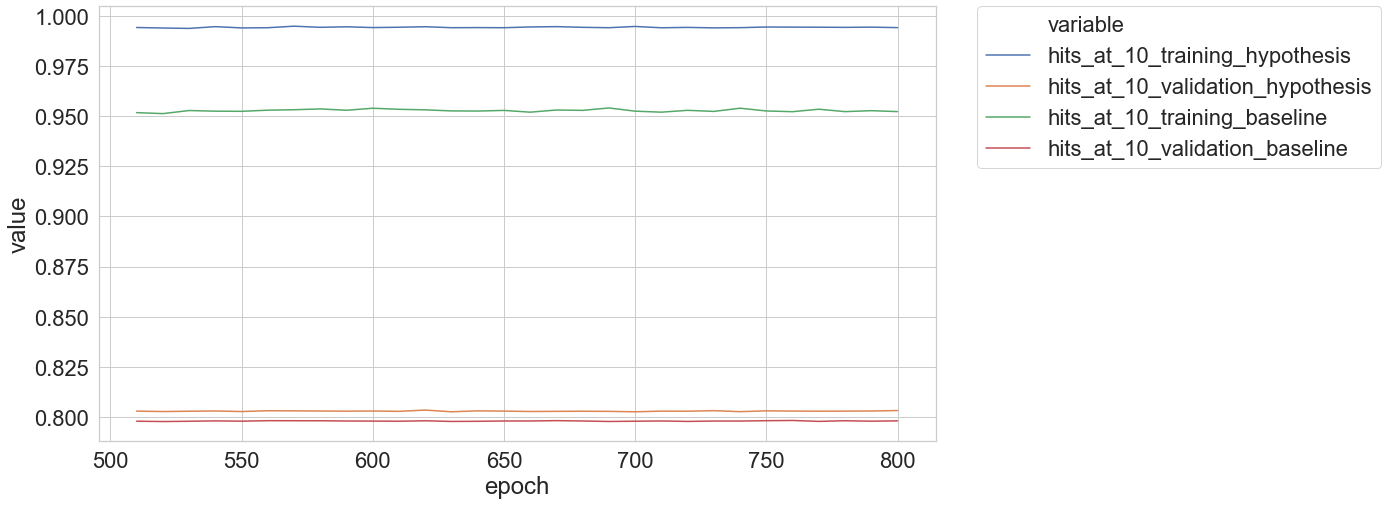
\includegraphics[width=0.45\textwidth, height=0.2\textheight]{FB15k_hits_at_10_Results_Clipped}
		}
\end{figure}

% Hits@3

\begin{figure}[H]
	\parbox{.5\linewidth}{
   		\caption{WN18 Hits@3}
   		\centering
    		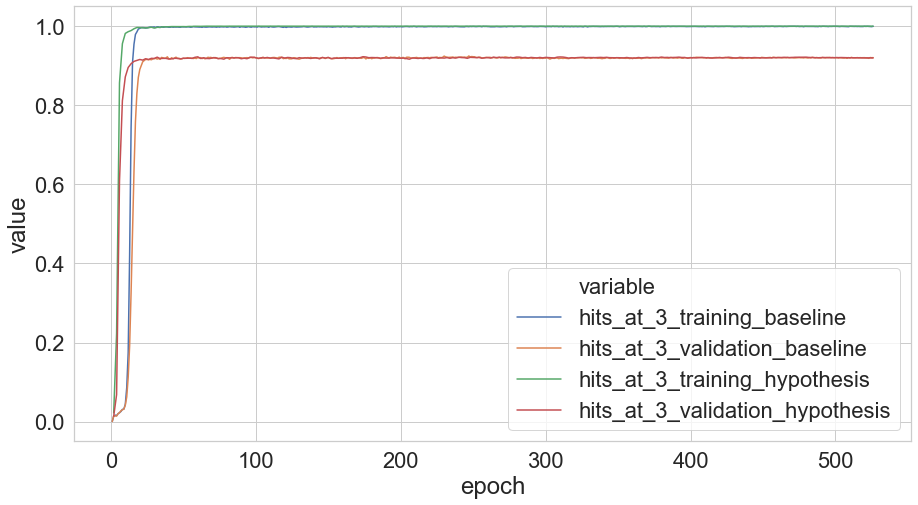
\includegraphics[width=0.45\textwidth, height=0.2\textheight]{WN18_hits_at_3_Results}
		}
	\hfill
	\parbox{.5\linewidth}{
		\caption{FB15k Hits@3}
   		\centering
		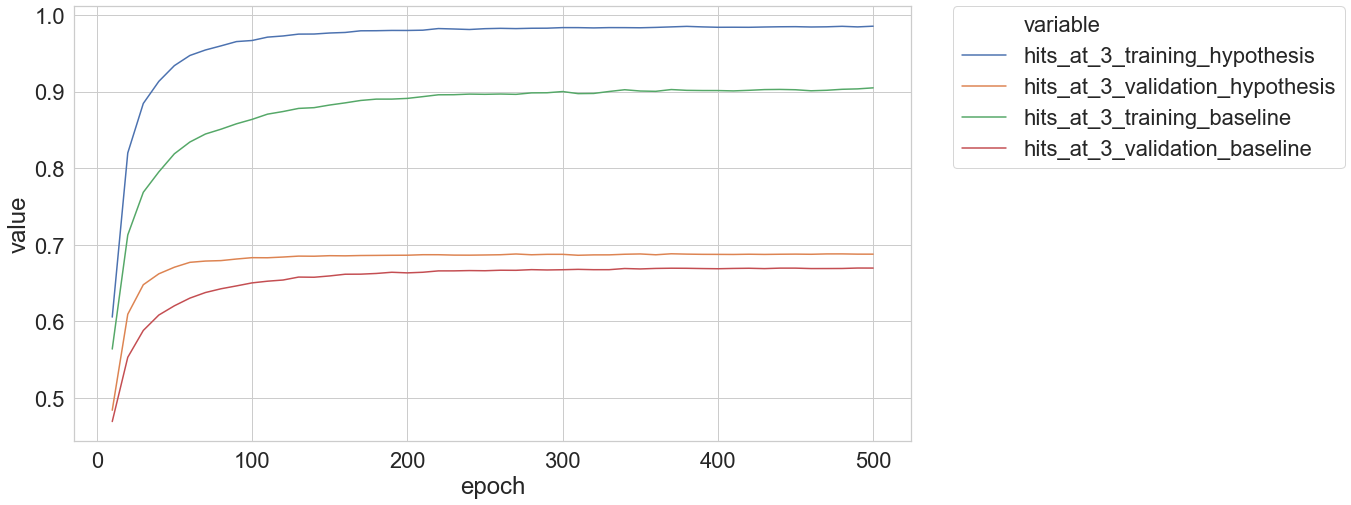
\includegraphics[width=0.45\textwidth, height=0.2\textheight]{FB15k_hits_at_3_Results}
		}
\end{figure}

\begin{figure}[H]
	\parbox{.5\linewidth}{
   		\caption{WN18 Hits@3 Clipped View}
   		\centering
    		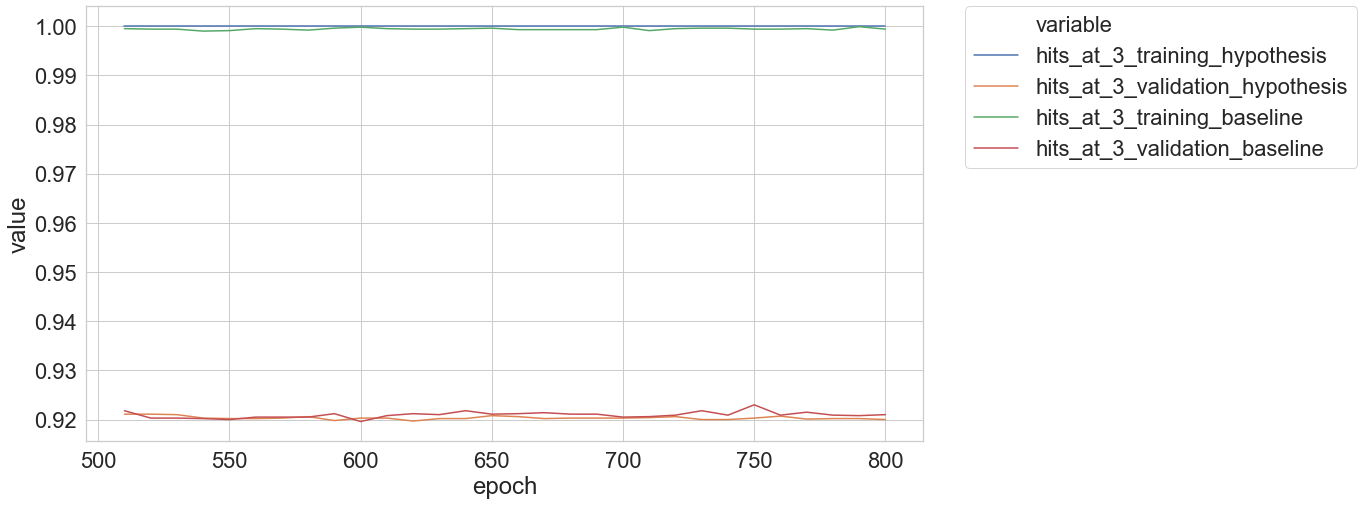
\includegraphics[width=0.45\textwidth, height=0.2\textheight]{WN18_hits_at_3_Results_Clipped}
		}
	\hfill
	\parbox{.5\linewidth}{
		\caption{FB15k Hits@3  Clipped View}
   		\centering
		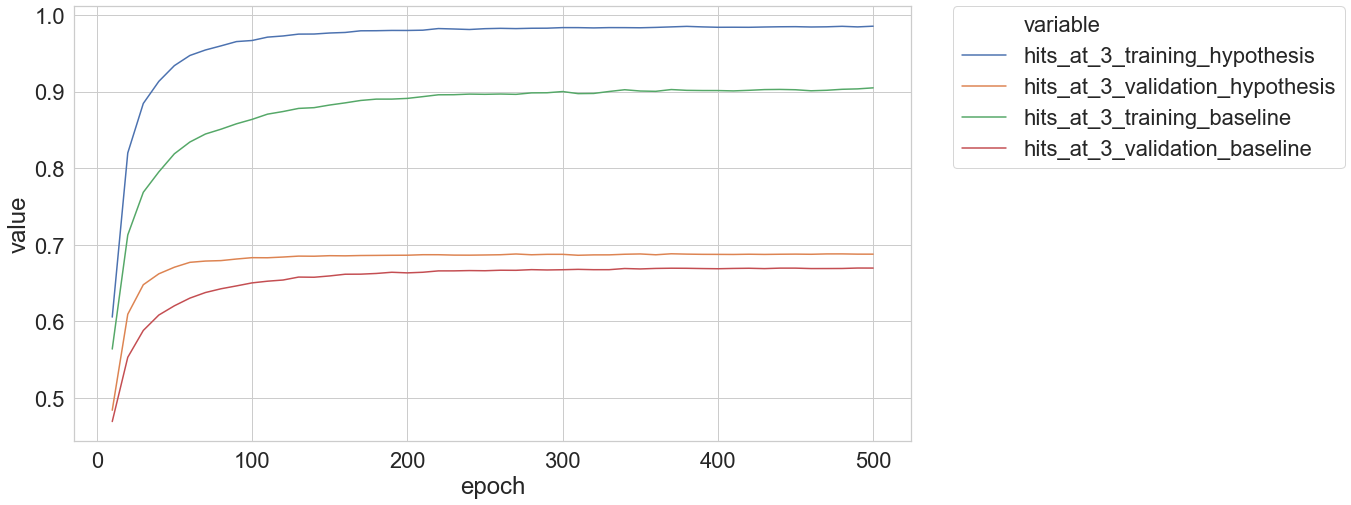
\includegraphics[width=0.45\textwidth, height=0.2\textheight]{FB15k_hits_at_3_Results_Clipped}
		}
\end{figure}

% Hits@1

\begin{figure}[H]
	\parbox{.5\linewidth}{
   		\caption{WN18 Hits@1}
   		\centering
    		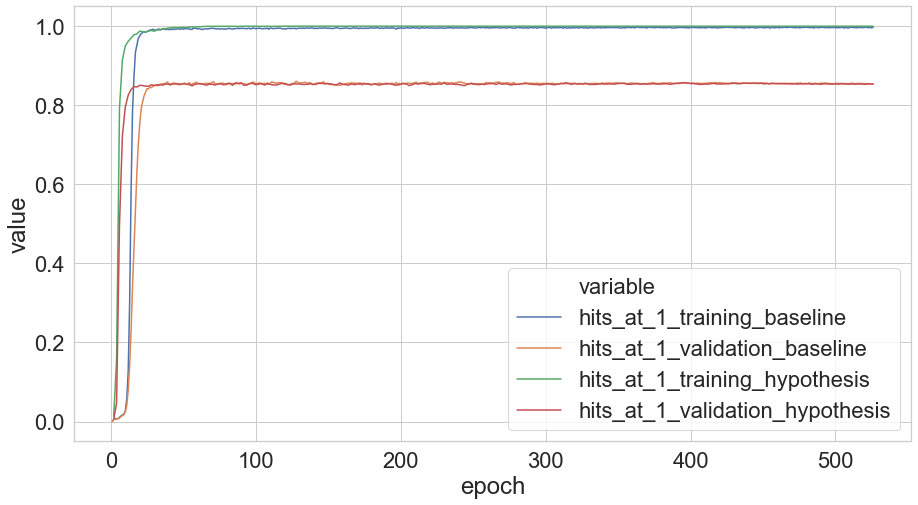
\includegraphics[width=0.45\textwidth, height=0.2\textheight]{WN18_hits_at_1_Results}
		}
	\hfill
	\parbox{.5\linewidth}{
		\caption{FB15k Hits@1}
   		\centering
		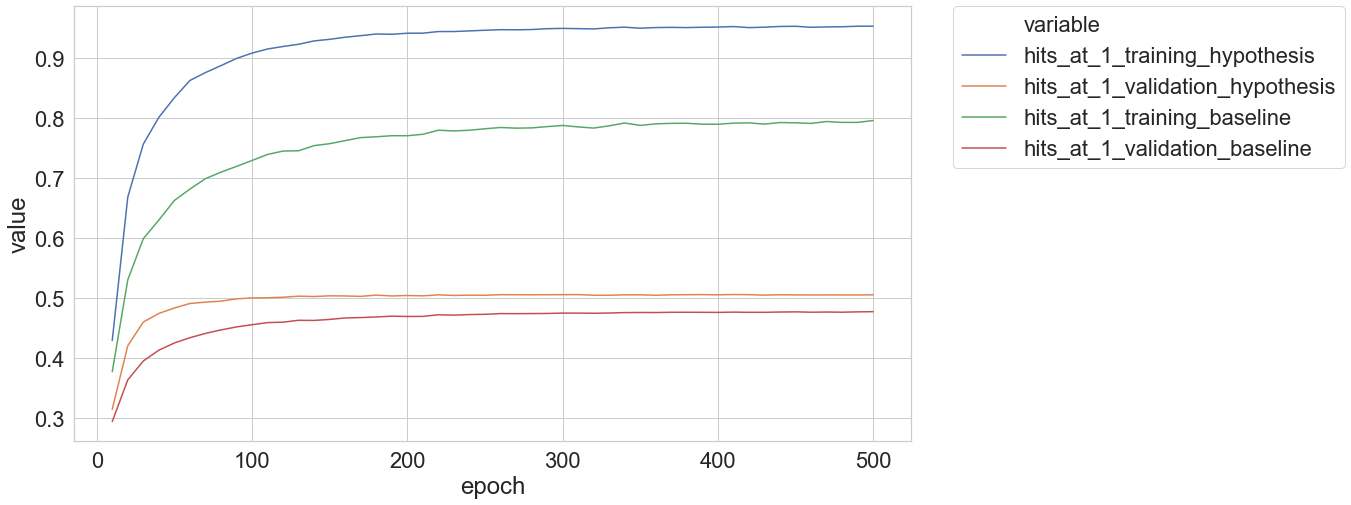
\includegraphics[width=0.45\textwidth, height=0.2\textheight]{FB15k_hits_at_1_Results}
		}
\end{figure}

\begin{figure}[H]
	\parbox{.5\linewidth}{
   		\caption{WN18 Hits@1 Clipped View}
   		\centering
    		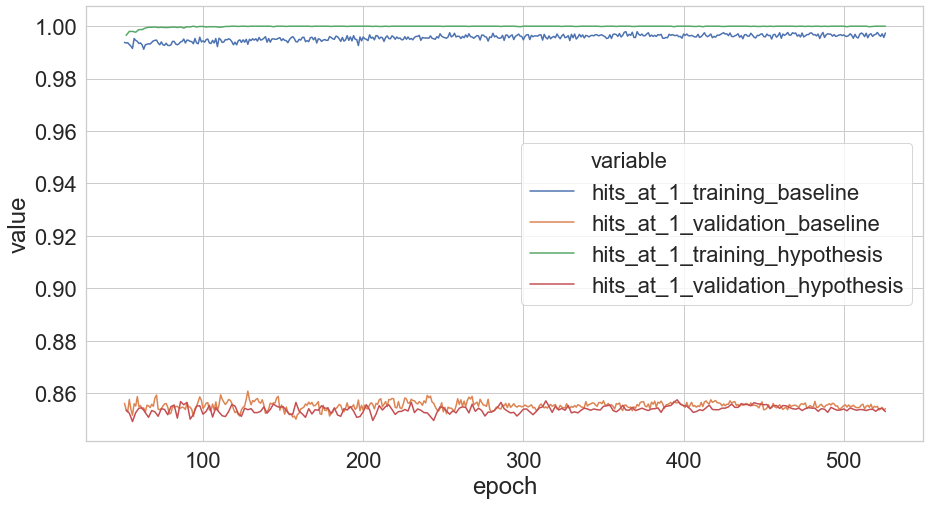
\includegraphics[width=0.45\textwidth, height=0.2\textheight]{WN18_hits_at_1_Results_Clipped}
		}
	\hfill
	\parbox{.5\linewidth}{
		\caption{FB15k Hits@1  Clipped View}
   		\centering
		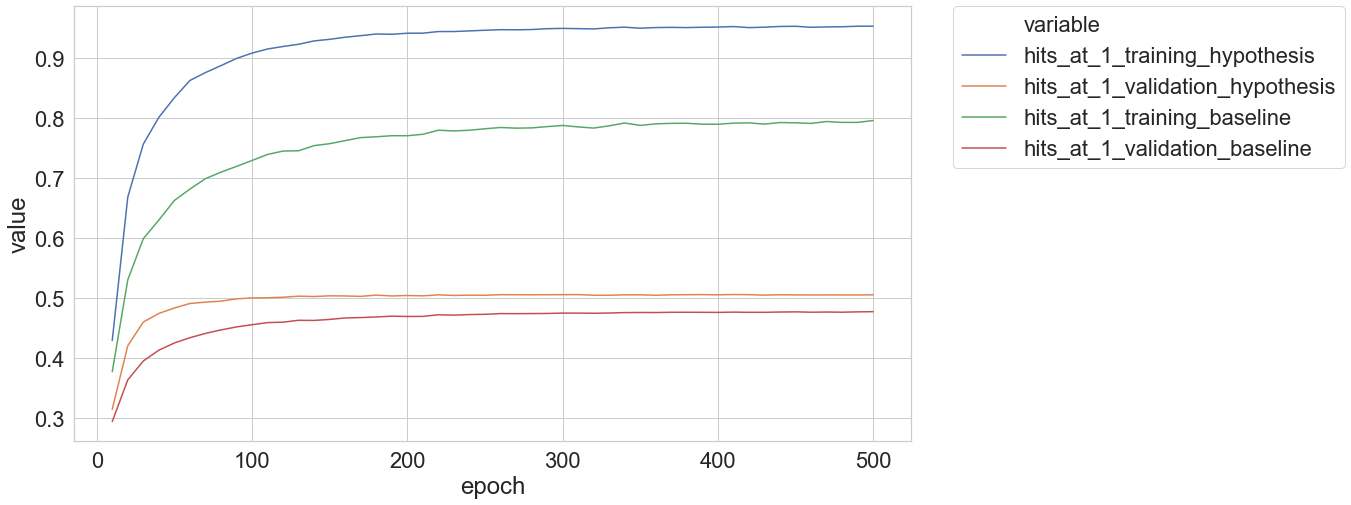
\includegraphics[width=0.45\textwidth, height=0.2\textheight]{FB15k_hits_at_1_Results_Clipped}
		}
\end{figure}

% Mean rank

\begin{figure}[H]
	\parbox{.5\linewidth}{
   		\caption{WN18 Mean Rank}
   		\centering
    		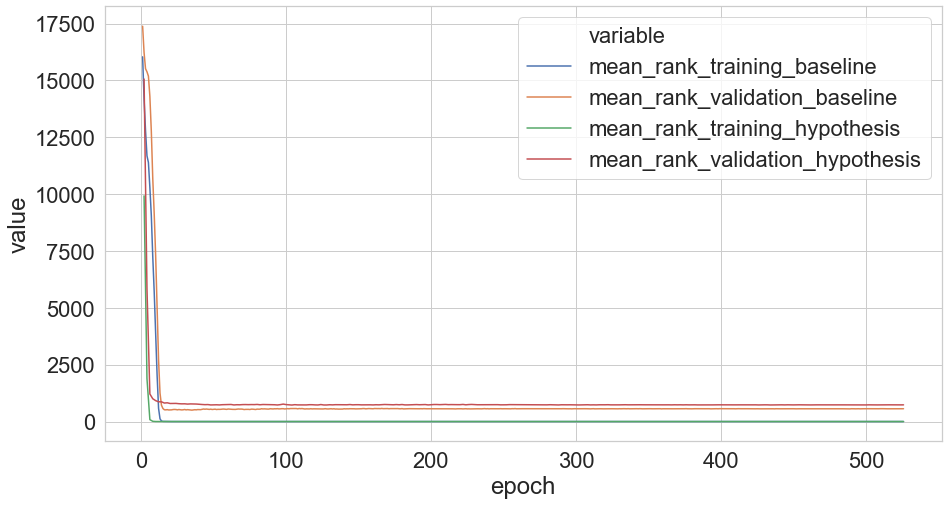
\includegraphics[width=0.45\textwidth, height=0.2\textheight]{WN18_mean_rank_Results}
		}
	\hfill
	\parbox{.5\linewidth}{
		\caption{FB15k Mean Rank}
   		\centering
		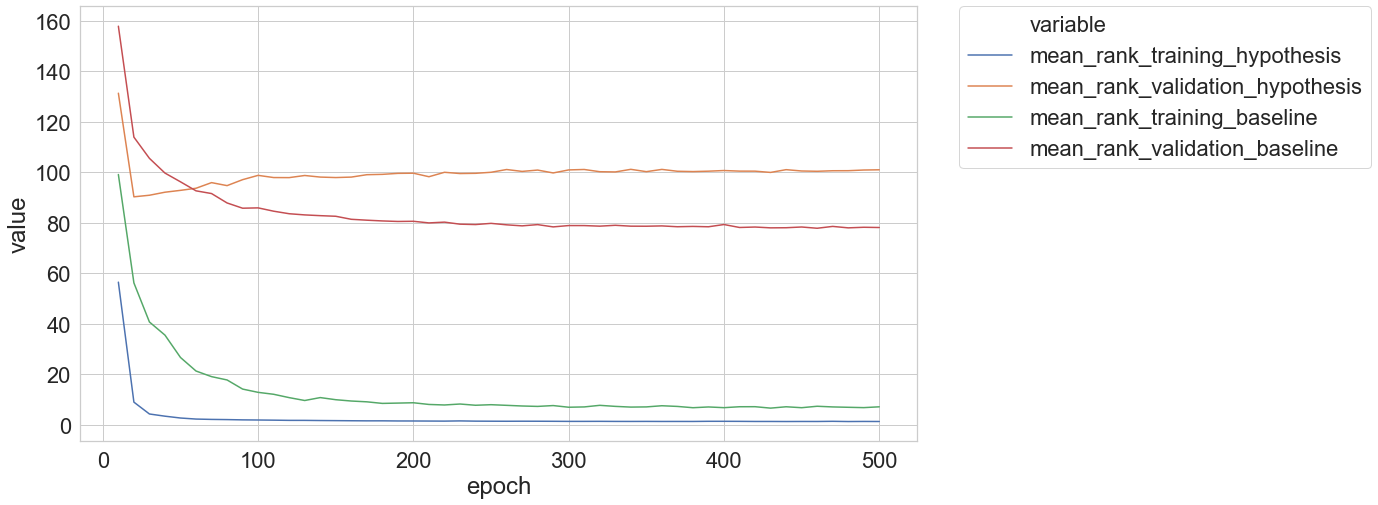
\includegraphics[width=0.45\textwidth, height=0.2\textheight]{FB15k_mean_rank_Results}
		}
\end{figure}

\begin{figure}[H]
	\parbox{.5\linewidth}{
   		\caption{WN18 Mean Rank Clipped View}
   		\centering
    		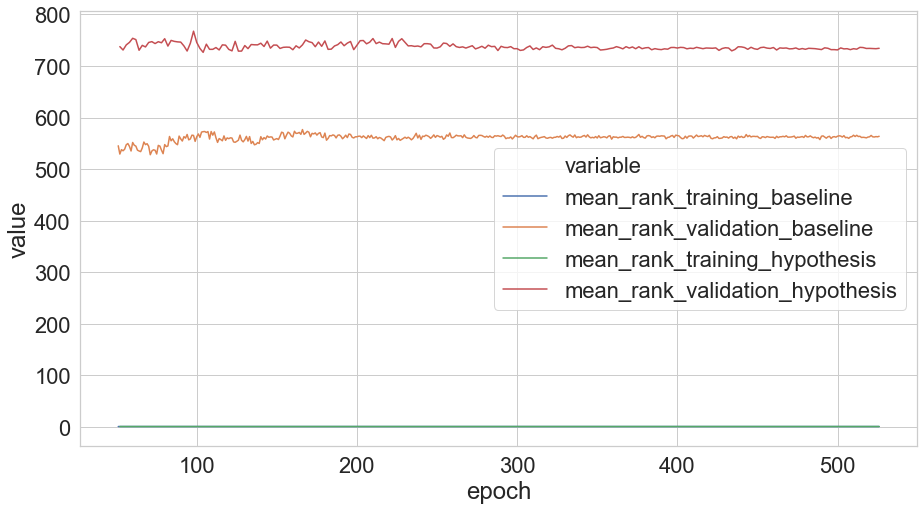
\includegraphics[width=0.45\textwidth, height=0.2\textheight]{WN18_mean_rank_Results_Clipped}
		}
	\hfill
	\parbox{.5\linewidth}{
		\caption{FB15k Mean Rank Clipped View}
   		\centering
		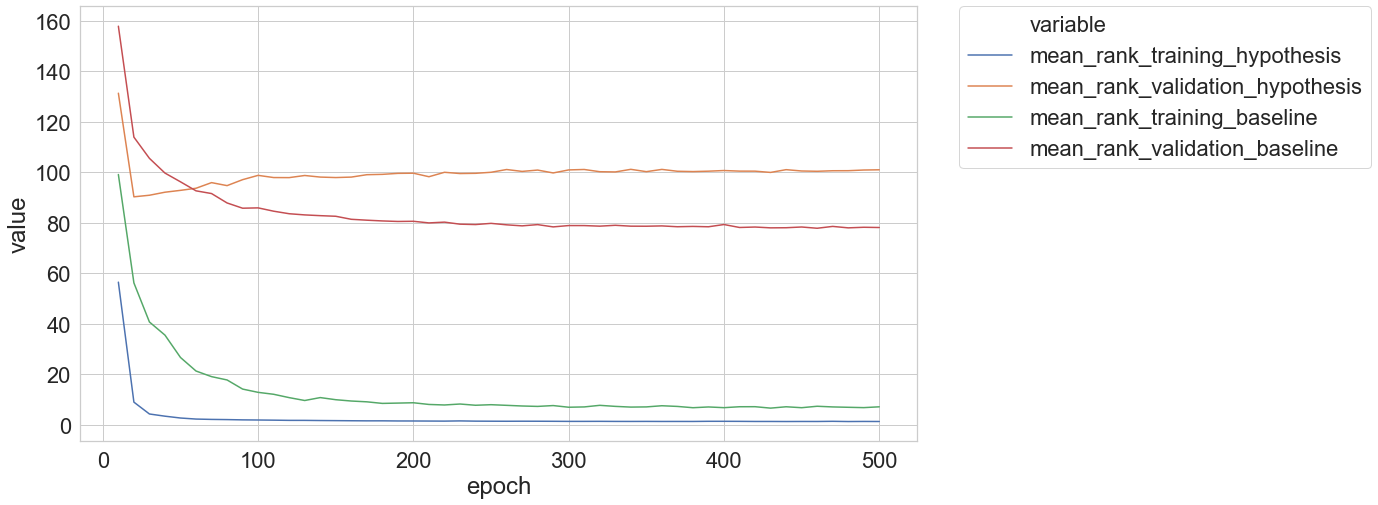
\includegraphics[width=0.45\textwidth, height=0.2\textheight]{FB15k_mean_rank_Results_Clipped}
		}
\end{figure}

% Mean reciprocal rank

\begin{figure}[H]
	\parbox{.5\linewidth}{
   		\caption{WN18 Mean Reciprocal Rank}
   		\centering
    		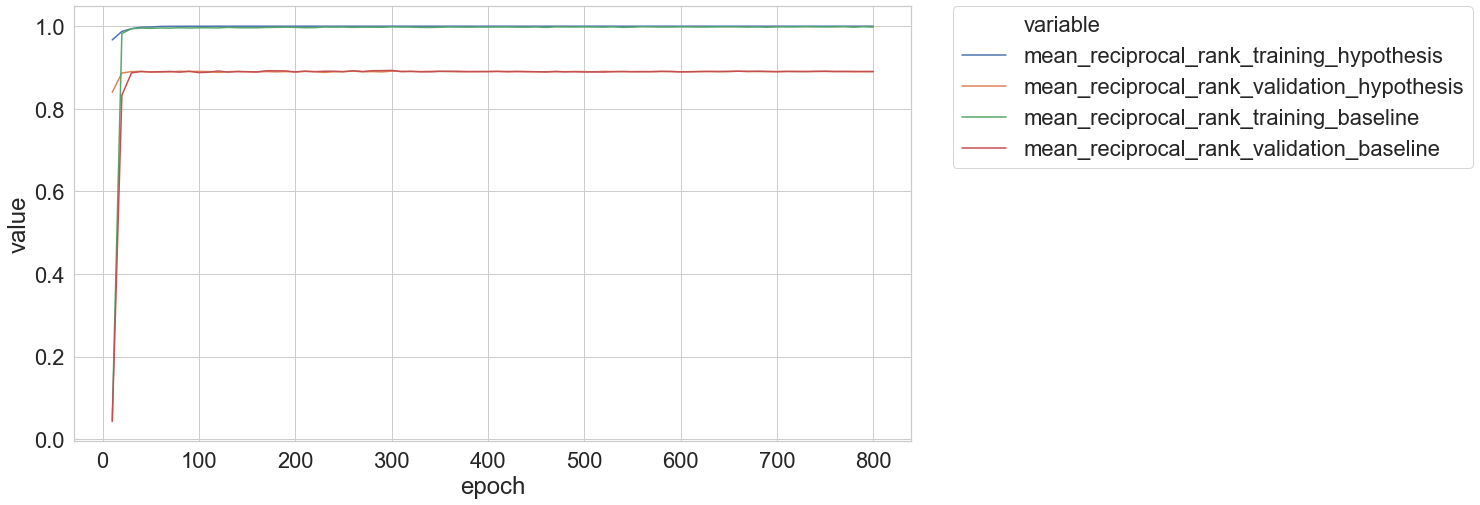
\includegraphics[width=0.45\textwidth, height=0.2\textheight]{WN18_mean_reciprocal_rank_Results}
		}
	\hfill
	\parbox{.5\linewidth}{
		\caption{FB15k Mean Reciprocal Rank}
   		\centering
		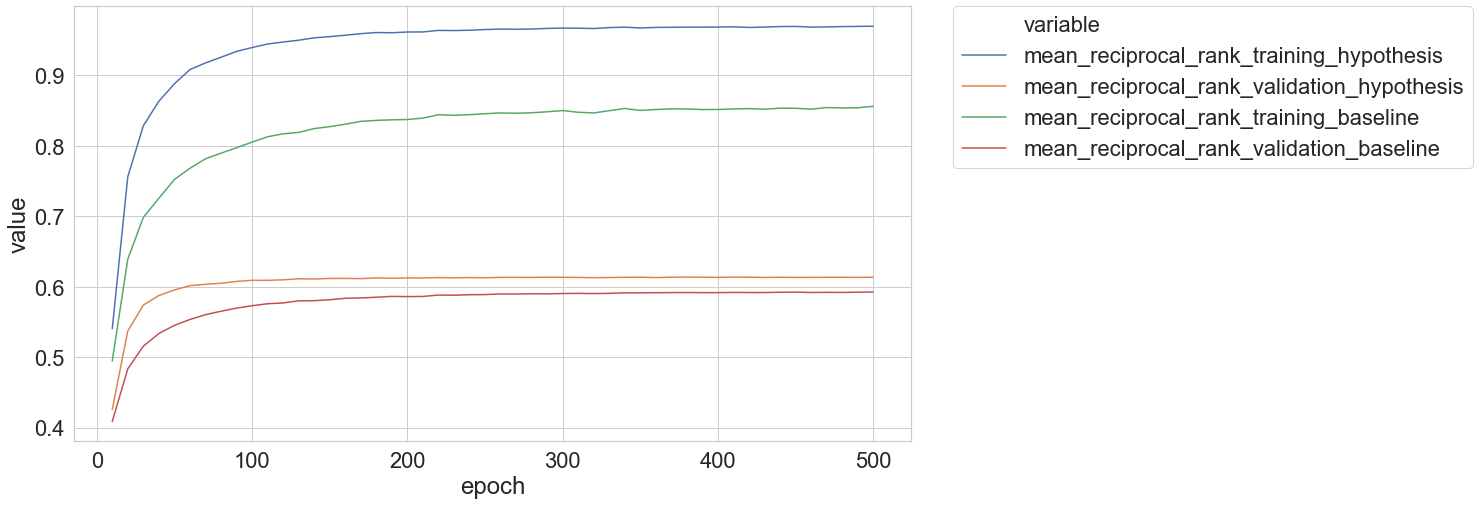
\includegraphics[width=0.45\textwidth, height=0.2\textheight]{FB15k_mean_reciprocal_rank_Results}
		}
\end{figure}

\begin{figure}[H]
	\parbox{.5\linewidth}{
   		\caption{WN18 Mean Reciprocal Rank Clipped View}
   		\centering
    		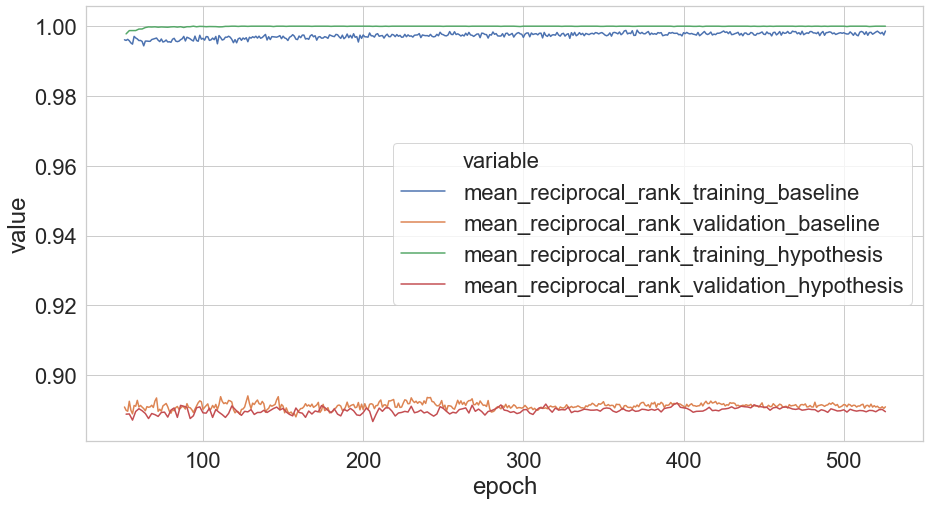
\includegraphics[width=0.45\textwidth, height=0.2\textheight]{WN18_mean_reciprocal_rank_Results_Clipped}
		}
	\hfill
	\parbox{.5\linewidth}{
		\caption{FB15k Mean Reciprocal Rank Clipped View}
   		\centering
		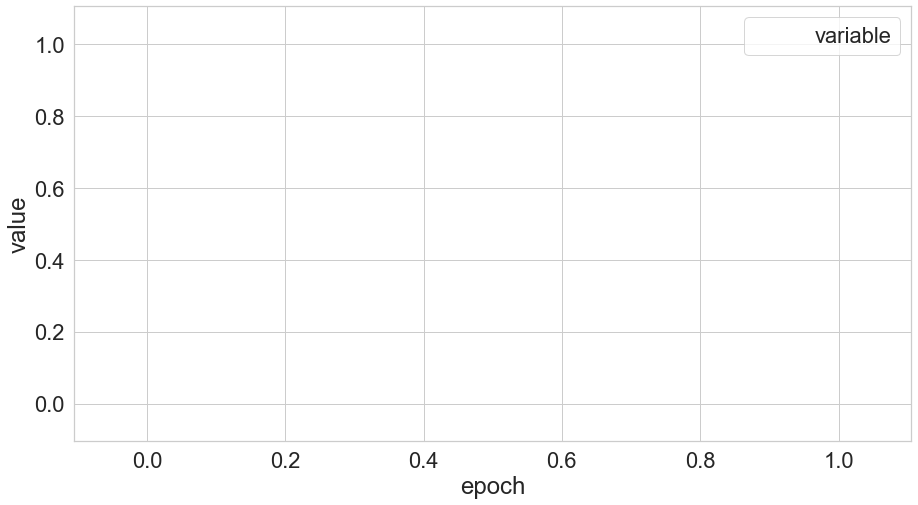
\includegraphics[width=0.45\textwidth, height=0.2\textheight]{FB15k_mean_reciprocal_rank_Results_Clipped}
		}
\end{figure}

% Test results

\begin{table}[H]
	\parbox{.5\linewidth}{
		\caption{Link prediction results on WN18}
		\centering
		\resizebox{0.5\columnwidth}{!}{%
		\begin{tabular}{lllllllllll}
  			\textbf{Model} & \textbf{H@10} & \textbf{H@3} & \textbf{H@1} & \textbf{MR} & \textbf{MRR} \\
  			\hline
  			TransE (Bordes et al. 2013) & .892 & - & - & \textbf{251} & - \\
  			DistMult (Yang et al. 2015) & .936 & .914 & .728 & 902 & .822 \\
  			ComplEx (Trouillon et al. 2016) & .947 & .936 & .936 & - & .941 \\
  			ANALOGY (Liu, Wu, and Yang 2017) & .947 & .944 & .939 & - & .942 \\
  			Neural LP (Yang, Yang, and Cohen 2017) & .945 & - & - & - & .940 \\
			R-GCN (Schlichtkrull et al. 2018) & \textbf{.964} & .929 & .697 & - & .819 \\
			TorusE (Ebisu and Ichise 2018) & .954 & .950 & .943 & - & .947 \\
			ConvE (Dettmers et al. 2018) & .956 & .946 & .935 & 374 & .943 \\
			HypER (Bala\v{z}evi\'c et al. 2019) & .958 & \textbf{.955} & \text{.947} & 431 & \textbf{.951} \\
  			\hline
  			HypER+ (ours) & .957 & .953 & .945 & 599 & .949 \\
		\end{tabular}%
		}}
	\hfill
	\parbox{.5\linewidth}{
	\caption{Link prediction results on FB15k}
		\centering
		\resizebox{0.5\columnwidth}{!}{%
		\begin{tabular}{lllllllllll}
  			\textbf{Model} & \textbf{H@10} & \textbf{H@3} & \textbf{H@1} & \textbf{MR} & \textbf{MRR} \\
  			\hline
  			TransE (Bordes et al. 2013) & .471 & - & - & 125 & - \\
  			DistMult (Yang et al. 2015) & .824 & .733 & .546 & 97 & .654 \\
  			ComplEx (Trouillon et al. 2016) & .840 & .759 & .599 & - & .692 \\
  			ANALOGY (Liu, Wu, and Yang 2017) & .854 & .785 & .646 & - & .725 \\
  			Neural LP (Yang, Yang, and Cohen 2017) & .837 & - & - & - & .760 \\
			R-GCN (Schlichtkrull et al. 2018) & .842 & .760 & .601 & - & .696 \\
			TorusE (Ebisu and Ichise 2018) & .832 & .771 & .674 & - & .733\\
			ConvE (Dettmers et al. 2018) & .831 & .723 & .558 & 51 & .657 \\
			HypER (Bala\v{z}evi\'c et al. 2019) & .885 & .829 & .734 & \textbf{44} & .790 \\
  			\hline
  			HypER+ (ours) & \textbf{.894} & \textbf{.856} & \textbf{.790} & 79 & \textbf{.829} \\
		\end{tabular}%
		}}
\end{table}

\section{HypER+ with Pre-Trained Word Embeddings}

\subsubsection{Model Summary} 
In order to overcome the expressiveness problems evident in the Freebase test dataset, more nonlinear relational factorisation approaches have been proposed \cite{ComplEx, Neural LP, TorusE}. \newline
HypER is a model that uses convolutional relational filters r that are convolved with the subject entity e1, producing an intermediate relational representation. The dot product of the relational representation is then taken with the object entity e2 to produce relation-specific score between the two entities. The HypER model only produces a latent relational representation for the subject entity e1, we extend this model to also produce a relational representation for the object entity e2, and call this model HpyER+. HypER+ thus produces entity-relational representations that approximate KG spacial locality. \newline
\subsubsection{Binary Cross Entropy Loss}
The binary cross entropy loss \cite{reference} is used to train the HypER+ model. Like the RNTN model, the input consists of an entity-relational pair, where the entity is a subject entity and an object entity is presented as a target to complete the triple. A logit is generated for each sample and passed through through a logarithmic sigmoid or softmax function. Loss is generated by comparing the produced likelihood with the expected likelihood, 0 or 1. The sum of all losses is aggregated and back propagated through the network for parameter update. \newline

\subsubsection{Experimental Setup} 

We use the following benchmark knowledge graphs: WN18RR is a subset of WN18, created by Dettmers et al. by removing the inverse relations from WN18. WN18RR contains 40,943 entities and 11 relations. \newline
FB15k-237 - was created by Toutanova et al., noting that the validation and test sets of FB15k and WN18 contain the inverse of many relations present in the training set, making it easy for simple models to do well. FB15k-237 is a subset of FB15k with the inverse relations removed. It contains 14,541 entities and 237 relations. \newline \newline
Visualisations of the respective knowledge graphs are presented below:

\begin{figure}[H]
  	\caption{WN18RR Entities and Relations Graphplot}
   	\centering
    	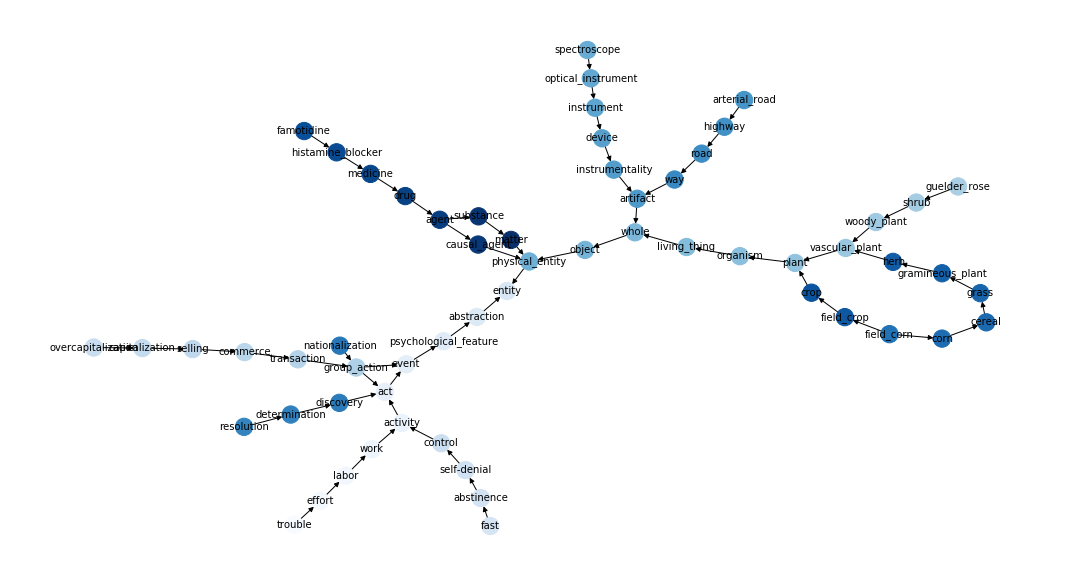
\includegraphics[width=\textwidth]{WN18RR_Graph}
\end{figure}

\begin{figure}[H]
  	\caption{FB15k-237 Entity and Relations Graphplot}
   	\centering
    	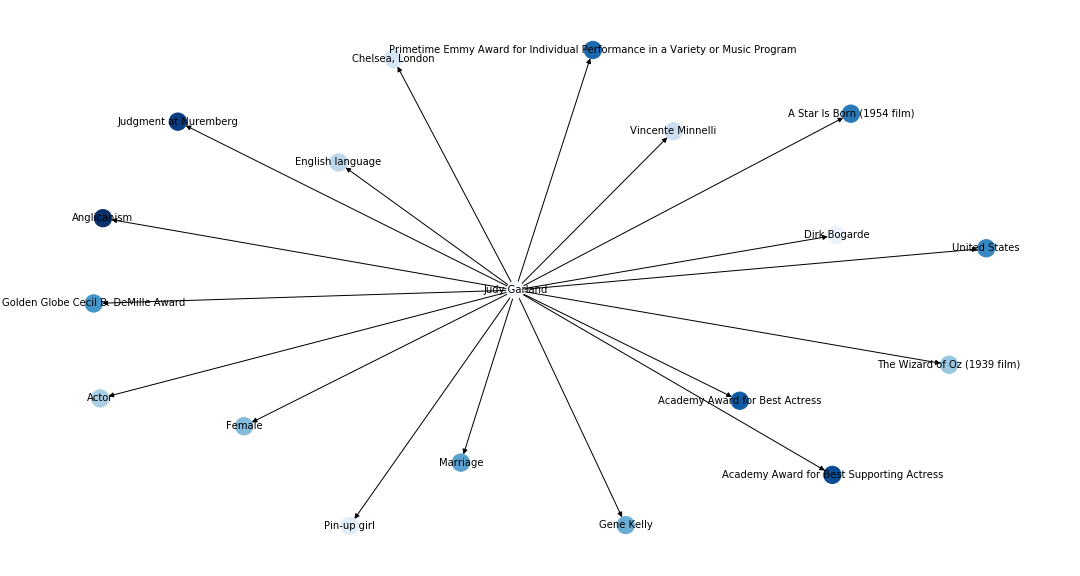
\includegraphics[width=\textwidth]{FB15k-237_Graph}
\end{figure}


We used the Pytorch framework to develop our model. This model is built on top of the HypER+ model introduced by (Magangane, Luyolo, and Brink, Wille 2019) ~\citep{magangane2019hyperplus}.  Glove pre-trained word vectors are used to initialise entity and relational embeddings for model training. These embeddings are dynamically adjusted during the training process to generate latent representations specific to the knowledge domain. Property counts for the respective knowledge graphs are presented below:

\begin{figure}[H]
	\parbox{.5\linewidth}{
   		\caption{WN18RR Property Barplot}
   		\centering
    		\includegraphics[width=0.45\textwidth]{WN18RR_Counts}
		}
	\hfill
	\parbox{.5\linewidth}{
		\caption{FB15k-237 Property Barplot}
   		\centering
    		\includegraphics[width=0.45\textwidth]{FB15k-237_Counts}
		}
\end{figure}


\begin{table}[H]
	\parbox{.5\linewidth}{
		\caption{WN18RR Property Counts}
		\centering
		\begin{tabular}{lllllllllll}
  			\textbf{Property} & \textbf{Count}  \\
  			\hline
  			Entities & 40,943  \\
  			Relations & 11  \\
  			Triples & 93,003 \\
		\end{tabular}
		}
	\hfill
	\parbox{.5\linewidth}{
		\caption{FB15k-237 Property Counts}
		\centering
		\begin{tabular}{lllllllllll}
  			\textbf{Property} & \textbf{Count}  \\
  			\hline
  			Entities & 14,541   \\
  			Relations & 237  \\
  			Triples & 310,116  \\
		\end{tabular}
		}
\end{table}


Summary statistics of the respective knowledge graphs Resource Description Framework (RDF) decomposition - subject, predicate, object - are presented below:

% Predicate

\begin{figure}[H]
	\parbox{.5\linewidth}{
   		\caption{WN18RR Predicate Barplot}
   		\centering
    		\includegraphics[width=0.45\textwidth, height=0.2\textheight]{WN18RR_Predicate_Counts}
		}
	\hfill
	\parbox{.5\linewidth}{
		\caption{FB15k-237 Predicate Barplot}
   		\centering
		\includegraphics[width=0.45\textwidth, height=0.2\textheight]{FB15k-237_Predicate_Counts}
		}
\end{figure}

\begin{table}[H]
	\parbox{.5\linewidth}{
		\caption{WN18RR Predicate Statistics}
		\centering
		\begin{tabular}{lllllllllll}
  			\textbf{Statistic} & \textbf{Value}  \\
  			\hline
			Count & 11 \\
			Max & 37,221  \\
			Min & 86 \\
  			Median & 3150  \\
  			IQR & 5433.5  \\
		\end{tabular}
		}
	\hfill
	\parbox{.5\linewidth}{
		\caption{FB15k-237 Predicate Statistics}
		\centering
		\begin{tabular}{lllllllllll}
  			\textbf{Statistic} & \textbf{Value}  \\
  			\hline
			Count & 237 \\
			Max & 16,391 \\
			Min & 45  \\
  			Median & 426  \\
  			IQR & 819 \\
		\end{tabular}
		}
\end{table}

% Subject

\begin{figure}[H]
	\parbox{.5\linewidth}{
   		\caption{WN18RR Subject Barplot}
   		\centering
    		\includegraphics[width=0.45\textwidth, height=0.2\textheight]{WN18RR_Subject_Counts}
		}
	\hfill
	\parbox{.5\linewidth}{
		\caption{FB15k-237 Subject Barplot}
   		\centering
		\includegraphics[width=0.45\textwidth, height=0.2\textheight]{FB15k-237_Subject_Counts}
		}
\end{figure}


\begin{table}[H]
	\parbox{.5\linewidth}{
		\caption{WN18RR Subject Statistics}
		\centering
		\begin{tabular}{lllllllllll}
  			\textbf{Statistic} & \textbf{Value}  \\
  			\hline
			Count & 32,349 \\
			Max & 494 \\
			Min & 1 \\
  			Median & 2 \\
  			IQR & 2 \\
		\end{tabular}
		}
	\hfill
	\parbox{.5\linewidth}{
		\caption{FB15k-237 Subject Statistics}
		\centering
		\begin{tabular}{lllllllllll}
  			\textbf{Statistic} & \textbf{Value}  \\
  			\hline
			Count &13,891 \\
			Max & 1,518 \\
			Min & 1 \\
  			Median & 16 \\
  			IQR & 20 \\
		\end{tabular}
		}
\end{table}

% Object

\begin{figure}[H]
	\parbox{.5\linewidth}{
   		\caption{WN18RR Object Barplot}
   		\centering
    		\includegraphics[width=0.45\textwidth, height=0.2\textheight]{WN18RR_Object_Counts}
		}
	\hfill
	\parbox{.5\linewidth}{
		\caption{FB15k-237 Object Barplot}
   		\centering
		\includegraphics[width=0.45\textwidth, height=0.2\textheight]{FB15k-237_Object_Counts}
		}
\end{figure}


\begin{table}[H]
	\parbox{.5\linewidth}{
		\caption{WN18RR Object Statistics}
		\centering
		\begin{tabular}{lllllllllll}
  			\textbf{Statistic} & \textbf{Value}  \\
  			\hline
			Count & 26,162 \\
			Max & 514 \\
			Min & 1 \\
  			Median & 1 \\
  			IQR & 2 \\
		\end{tabular}
		}
	\hfill
	\parbox{.5\linewidth}{
		\caption{FB15k-237 Object Statistics}
		\centering
		\begin{tabular}{lllllllllll}
  			\textbf{Statistic} & \textbf{Value}  \\
  			\hline
			Count & 13,504 \\
			Max & 7,124 \\
			Min & 1 \\
  			Median & 10 \\
  			IQR & 16 \\
		\end{tabular}
		}
\end{table}

For WN18RR, it can be seen that relations are skewed toward the relations "hypernym" and "derivationally related from", with a maximum of 37,221 occurrences, with an IQR of 5433.5 and 819 respectively. \newline
FB15k-237 are skewed toward film relations. We would expect reasonable performance across this type of relation for the knowledge graph. \newline
WN18R and FB15k-237 subjects are somewhat uniform aside from a small number of high occurrences entities, with the median number of occurrences is 3 and 16 respectively, and with an IQR of 2 and 20 respectively. 
WN18RR object occurrences are somewhat uniform. FB15k-237 object occurrences are skewed, with the "United States" partaking in the highest number of facts. This is in comparison to a median object occurrence of 1 and an interquartile range of 10,
and an IQR of 2 and 16 respectively. \newline
Such high variance in FB15k-237 suggests poor potential model performance for FB15k-237 relative to WN18RR.  

% Pre-Trained Word Embeddings

\subsubsection{Hypothesis 3: \newline 
HypER+ with Glove Word Embeddings}
HypER+ here is implemented using Glove pre-trained word embeddings. \newline
The the model was trained on Google Cloud Platform, on a N1 series instance with  8 CPU cores, 30GB RAM, 512GB SSD and a Nvidia Tesla P100 GPU. \newline
We evaluate the model using standard link prediction benchmarks. \newline 
Code to reproduce: https://github.com/xhosaBoy/HypER-Pretrained-Word-Vectors \newline
Baseline: https://github.com/xhosaBoy/HypER-baseline

\subsubsection{Word Embeddings}
Previous work represented entities and relations as randomly initialised vector representations. We show that performance can be improved when entities and relations are represented as an average of their constituting word vectors. 
This allows sharing of statistical strength between, for instance, facts involving the “Michael Jackson” and “Musician” We demonstrate that the HypER+ model improves across all knowledge grpahs when these word vectors are initialized 
with vectors learned from unsupervised large corpora, namely the Glove language model.

\subsubsection{Link Prediction Results}
The link prediction benchmark results of the HypER+ with pre-trained embeddings model, compared against other link prediction models, are presented below:

% Cost

\begin{figure}[H]
	\parbox{.5\linewidth}{
   		\caption{WN18RR Cost}
   		\centering
    		\includegraphics[width=0.45\textwidth, height=0.2\textheight]{WN18RR_Cost_Results}
		}
	\hfill
	\parbox{.5\linewidth}{
		\caption{FB15k-237 Cost}
   		\centering
		\includegraphics[width=0.45\textwidth, height=0.2\textheight]{FB15k-237_Cost_Results}
		}
\end{figure}

\begin{figure}[H]
	\parbox{.5\linewidth}{
   		\caption{WN18RR Cost Clipped View}
   		\centering
    		\includegraphics[width=0.45\textwidth, height=0.2\textheight]{WN18RR_Cost_Results_Clipped}
		}
	\hfill
	\parbox{.5\linewidth}{
		\caption{FB15k-237 Cost Clipped View}
   		\centering
		\includegraphics[width=0.45\textwidth, height=0.2\textheight]{FB15k-237_Cost_Results_Clipped}
		}
\end{figure}

% Hits@10

\begin{figure}[H]
	\parbox{.5\linewidth}{
   		\caption{WN18RR Hits@10}
   		\centering
    		\includegraphics[width=0.45\textwidth, height=0.2\textheight]{WN18RR_hits_at_10_Results}
		}
	\hfill
	\parbox{.5\linewidth}{
		\caption{FB15k-237 Hits@10}
   		\centering
		\includegraphics[width=0.45\textwidth, height=0.2\textheight]{FB15k-237_hits_at_10_Results}
		}
\end{figure}

\begin{figure}[H]
	\parbox{.5\linewidth}{
   		\caption{WN18RR Hits@10 Clipped View}
   		\centering
    		\includegraphics[width=0.45\textwidth, height=0.2\textheight]{WN18RR_hits_at_10_Results_Clipped}
		}
	\hfill
	\parbox{.5\linewidth}{
		\caption{FB15k-237 Hits@10  Clipped View}
   		\centering
		\includegraphics[width=0.45\textwidth, height=0.2\textheight]{FB15k-237_hits_at_10_Results_Clipped}
		}
\end{figure}

% Hits@3

\begin{figure}[H]
	\parbox{.5\linewidth}{
   		\caption{WN18RR Hits@3}
   		\centering
    		\includegraphics[width=0.45\textwidth, height=0.2\textheight]{WN18RR_hits_at_3_Results}
		}
	\hfill
	\parbox{.5\linewidth}{
		\caption{FB15k-237 Hits@3}
   		\centering
		\includegraphics[width=0.45\textwidth, height=0.2\textheight]{FB15k-237_hits_at_3_Results}
		}
\end{figure}

\begin{figure}[H]
	\parbox{.5\linewidth}{
   		\caption{WN18RR Hits@3 Clipped View}
   		\centering
    		\includegraphics[width=0.45\textwidth, height=0.2\textheight]{WN18RR_hits_at_3_Results_Clipped}
		}
	\hfill
	\parbox{.5\linewidth}{
		\caption{FB15k-237 Hits@3  Clipped View}
   		\centering
		\includegraphics[width=0.45\textwidth, height=0.2\textheight]{FB15k-237_hits_at_3_Results_Clipped}
		}
\end{figure}

% Hits@1

\begin{figure}[H]
	\parbox{.5\linewidth}{
   		\caption{WN18RR Hits@1}
   		\centering
    		\includegraphics[width=0.45\textwidth, height=0.2\textheight]{WN18RR_hits_at_1_Results}
		}
	\hfill
	\parbox{.5\linewidth}{
		\caption{FB15k-237 Hits@1}
   		\centering
		\includegraphics[width=0.45\textwidth, height=0.2\textheight]{FB15k-237_hits_at_1_Results}
		}
\end{figure}

\begin{figure}[H]
	\parbox{.5\linewidth}{
   		\caption{WN18RR Hits@1 Clipped View}
   		\centering
    		\includegraphics[width=0.45\textwidth, height=0.2\textheight]{WN18RR_hits_at_1_Results_Clipped}
		}
	\hfill
	\parbox{.5\linewidth}{
		\caption{FB15k-237 Hits@1  Clipped View}
   		\centering
		\includegraphics[width=0.45\textwidth, height=0.2\textheight]{FB15k-237_hits_at_1_Results_Clipped}
		}
\end{figure}

% Mean rank

\begin{figure}[H]
	\parbox{.5\linewidth}{
   		\caption{WN18RR Mean Rank}
   		\centering
    		\includegraphics[width=0.45\textwidth, height=0.2\textheight]{WN18RR_mean_rank_Results}
		}
	\hfill
	\parbox{.5\linewidth}{
		\caption{FB15k-237 Mean Rank}
   		\centering
		\includegraphics[width=0.45\textwidth, height=0.2\textheight]{FB15k-237_mean_rank_Results}
		}
\end{figure}

\begin{figure}[H]
	\parbox{.5\linewidth}{
   		\caption{WN18RR Mean Rank Clipped View}
   		\centering
    		\includegraphics[width=0.45\textwidth, height=0.2\textheight]{WN18RR_mean_rank_Results_Clipped}
		}
	\hfill
	\parbox{.5\linewidth}{
		\caption{FB15k-237 Mean Rank Clipped View}
   		\centering
		\includegraphics[width=0.45\textwidth, height=0.2\textheight]{FB15k-237_mean_rank_Results_Clipped}
		}
\end{figure}

% Mean reciprocal rank

\begin{figure}[H]
	\parbox{.5\linewidth}{
   		\caption{WN18RR Mean Reciprocal Rank}
   		\centering
    		\includegraphics[width=0.45\textwidth, height=0.2\textheight]{WN18RR_mean_reciprocal_rank_Results}
		}
	\hfill
	\parbox{.5\linewidth}{
		\caption{FB15k-237 Mean Reciprocal Rank}
   		\centering
		\includegraphics[width=0.45\textwidth, height=0.2\textheight]{FB15k-237_mean_reciprocal_rank_Results}
		}
\end{figure}

\begin{figure}[H]
	\parbox{.5\linewidth}{
   		\caption{WN18RR Mean Reciprocal Rank Clipped View}
   		\centering
    		\includegraphics[width=0.45\textwidth, height=0.2\textheight]{WN18RR_mean_reciprocal_rank_Results_Clipped}
		}
	\hfill
	\parbox{.5\linewidth}{
		\caption{FB15k-237 Mean Reciprocal Rank Clipped View}
   		\centering
		\includegraphics[width=0.45\textwidth, height=0.2\textheight]{FB15k-237_mean_reciprocal_rank_Results_Clipped}
		}
\end{figure}

% Test results

\begin{table}[H]
	\parbox{.5\linewidth}{
		\caption{Link prediction results on WN18RR}
		\centering
		\resizebox{0.5\columnwidth}{!}{%
		\begin{tabular}{lllllllllll}
  			\textbf{Model} & \textbf{H@10} & \textbf{H@3} & \textbf{H@1} & \textbf{MR} & \textbf{MRR} \\
  			\hline
  			DistMult (Yang et al. 2015) & .490 & .440 & .390 & 5110 & .430 \\
  			ComplEx (Trouillon et al. 2016) & .510 & .460 & .410 & 5261 & .440 \\
  			Neural LP (Yang, Yang, and Cohen 2017) & - & - & - & - & - \\
			MINERVA (Das et al. 2018) & - & - & - & - & - \\
			ConvE (Dettmers et al. 2018) & .520 & .440 & .400 & 4187 & .430 \\
			HypER (Bala\v{z}evi\'c et al. 2019) & .522 & .477 & \textbf{.436} & 5798 & .465 \\
  			\hline
  			HypER+ (ours) & \textbf{.552} & \textbf{.481} & .432 & \textbf{1586} & \textbf{.471} \\
		\end{tabular}%
		}}
	\hfill
	\parbox{.5\linewidth}{
	\caption{Link prediction results on FB15k-237}
		\centering
		\resizebox{0.5\columnwidth}{!}{%
		\begin{tabular}{lllllllllll}
  			\textbf{Model} & \textbf{H@10} & \textbf{H@3} & \textbf{H@1} & \textbf{MR} & \textbf{MRR} \\
  			\hline
  			DistMult (Yang et al. 2015) & .419 & .263 & .155 & 254 & .241 \\
  			ComplEx (Trouillon et al. 2016) & .428 & .275 & .158 & 339 & .247 \\
  			Neural LP (Yang, Yang, and Cohen 2017) & .408 & - & - & - & .250 \\
			MINERVA (Das et al. 2018) & .456 & - & - & - & - \\
			ConvE (Dettmers et al. 2018) & .501 & .356 & .237 & 244 & .325 \\
			HypER (Bala\v{z}evi\'c et al. 2019) & .520 & \textbf{.376} & \textbf{.252} & 250 & .341 \\
  			\hline
  			HypER+ (ours) & \textbf{.524} & \textbf{.376} & \textbf{.252} & \textbf{213} & \textbf{.342} \\
		\end{tabular}%
		}}
\end{table}




